\documentclass[american,titlepage,oneside]{ntnuthesis}

\title{An NTNU Thesis \LaTeX{} Document Class}
\shorttitle{An NTNU Thesis Document Class}
\author{Community of Practice in Computer Science Education at NTNU}
\shortauthor{CoPCSE$@$NTNU}
\date{CC-BY \ntnuthesisdate}

\addbibresource{thesis.bib}
\addbibresource{references.bib} % from lit review


% From https://www.overleaf.com/learn/latex/Glossaries

\makeglossaries % Prepare for adding glossary entries


\newglossaryentry{latex}{
        name=latex,
        description={Is a mark up language specially suited for
scientific documents}
}

\newglossaryentry{bibliography}{
    name=bibliography,
    plural=bibliographies,
    description={A list of the books referred to in a scholarly work, typically printed as an appendix}
}

\newglossaryentry{maths}{
    name=mathematics,
    description={Mathematics is what mathematicians do}
}

\newglossaryentry{locode}{
    name=UN/LOCODE,
    description={Five-letter geographic coding scheme maintained by the UN. The codes are assigned to, among others, ports where the first to letters represents a country code and the remaining three represents a location}
}

\newglossaryentry{aivdm}{
    name=AIVDM/AIVDO,
    description={The protocol used by AIS messages where AIVDM contains data received from other vessels, and AIVDO contains data from the owner vessel}
}


% --------------------
% ----- Acronyms -----
% --------------------

\newacronym{phd}{PhD}{philosophiae doctor}
\newacronym{CoPCSE}{CoPCSE@NTNU}{Community of Practice in Computer ScienceEducation at NTNU}
\newacronym{gcd}{GCD}{Greatest Common Divisor}
\newacronym{mo}{MO}{Maritime Optima AS}
\newacronym{ais}{AIS}{Automatic Identification Systems}
\newacronym{gis}{GIS}{Geographical Information System}
\newacronym{imo}{IMO}{International Maritime Organization}
\newacronym{mmsi}{MMSI}{Maritime Mobile Service Identity}
\newacronym{ntnu}{NTNU}{Norwegian University of Technology and Science}
\newacronym{ml}{ML}{Machine learning}
\newacronym{gt}{GT}{Gross Tonnage}
\newacronym{cog}{COG}{Course Over Ground}
\newacronym{sog}{SOG}{Speed Over Ground}
\newacronym{rot}{ROT}{Rate of Turn}
\newacronym{eta}{ETA}{Estimated Time of Arrival}
\newacronym{sspd}{SSPD}{Symmetric Segment-Path Distance}
\newacronym{dbscan}{DBSCAN}{Density-based spatial clustering of applications with noise}
\newacronym{rf}{RF}{Random Forest}
\newacronym{knn}{k-NN}{k-Nearest Neighbor}
\newacronym{rnn}{RNN}{Recurrent Neural Network}
\newacronym{svm}{SVM}{Support Vector Machine}
 % add glossary and acronym lists before document

\usepackage{rotating}
\usepackage{longtable}


\begin{document}

\chapter*{Abstract}

This thesis develops a new approach for automating the cost impact of security incidents. The method is based on detecting security incidents in news articles and then using an event study to determine the change in stock price resulting from the security incident. The main finding is that TODO.
\chapter*{Sammendrag}

TODO

\tableofcontents
\listoffigures
\listoftables
\lstlistoflistings

\printglossary[type=\acronymtype] % Print acronyms
\printglossary                    % Print glossary

\newcommand{\paragraphheader}[1]{\paragraph{#1}\mbox{}\\}
\newcommand{\todo}[1]{{\color{olive}\textbf{TODO:}\color{olive}#1}} % items to do

\setlength{\parindent}{4em}
%\setlength{\parskip}{1em}

\chapter{Introduction}

Thesis introduction chapter test.

Test commit.

Over the years, several thesis templates for \LaTeX{} have been developed by different groups at NTNU\@. Typically, there have been local templates for given study programmes, or different templates for the different study levels – bachelor, master, and \acrshort{phd}.\footnote{see, e.g., \url{https://github.com/COPCSE-NTNU/bachelor-thesis-NTNU} and \url{https://github.com/COPCSE-NTNU/master-theses-NTNU}}

Based on this experience, the \acrfull{CoPCSE}\footnote{\url{https://www.ntnu.no/wiki/display/copcse/Community+of+Practice+in+Computer+Science+Education+Home}} is hereby offering a template that should in principle be applicable for theses at all study levels. It is closely based on the standard \LaTeX{} \texttt{report} document class as well as previous thesis templates. Since the central regulations for thesis design have been relaxed – at least for some of the historical university colleges now part of NTNU – the template has been simlified and put closer to the default \LaTeX{} look and feel.

The purpose of the present document is threefold. It should serve (i) as a description of the document class, (ii) as an example of how to use it, and (iii) as a thesis template.

\chapter{Background}

In this chapter, concepts and terminology relevant to the thesis is explained, mainly, technological foundations such as \acrfull{ais}, conceptual foundations such as \acrshort{ais}-based trajectories and trajectory similarity measurements, and techniques applied to predicting future destination ports of traveling vessels, namely, \acrfull{ml}.

\section{Concepts}

This section describes the broader concepts that are important to the thesis's solution and later discussions,

\subsection{Vessel voyage definition}
\label{sec:vessel_voyage_definition}

In order to effectively predict a vessel's future destination, or analyze voyage patterns in general, a vessel voyage must first be defined. This is a crucial concept to define as it would change the outcome of any prediction method that considers historical voyages. The main factor to decide on is when does a vessel arrive at a port, or what conditions must be true for a vessel to have arrived at a port.

There might be several different reasons for a vessel to visit a port, not all of which means that the port was the vessels final stop in a voyage. For instance, larger vessels traveling long distances, often have to bunker (refuel) at bunker ports between the port they loaded and the port they will unload at. In some cases, vessels anchor outside of such bunker ports awaiting to be refueled by bunker vessels, while in other cases they can reduce their speed and be refueled without ever stopping completely. Another common reason for vessels to physically stop moving is congestion in ports. Very often vessels of any size have to wait their turn before loading or unloading at busy ports. In these cases they might anchor closer to a different port while they wait for access, however, it is likely that they do not consider themselves arrived in these scenarios. In either case, whether vessels refueling at bunker ports, or stopping for other reasons, should be considered arrivals or not ultimately depends on the desired outcome of future predictions and context.

For the purpose of this thesis, a voyage is defined only when the vessel herself claims to be moored by reflecting this as a navigational status in the \acrfull{ais} data. As vessels usually do not use the moored signal when bunkering, or for short stops along a voyage, this entails that the proposed solution will be more prone to predicting the final destination of a vessel even though it might stop for other reasons along the voyage. This voyage is beneficial for actors in the industry who are interested in knowing what vessels are available in different regions for chartering, however, a disadvantage is that fewer voyages can be constructed from the available data as longer voyages could have been divided into multiple smaller voyages if considering, for instance, bunkering as port arrivals.

A literature study, later described in \cref{sec:lit_review}, shows that there are few studies that consider voyage prediction, however, the most common alternative method of defining trajectories of vessels is to use some manner of clustering. The most promising of these detected port arrivals by detecting clusters of vessel positions transmitted close to ports. In contrast to using navigational statuses, this method defined voyages as trajectories between stopping ports, thus voyages stopping mid-voyage at smaller ports was considered their own voyages.

\begin{figure}[htbp]  % order of priority: h here, t top, b bottom, p page
    \centering
    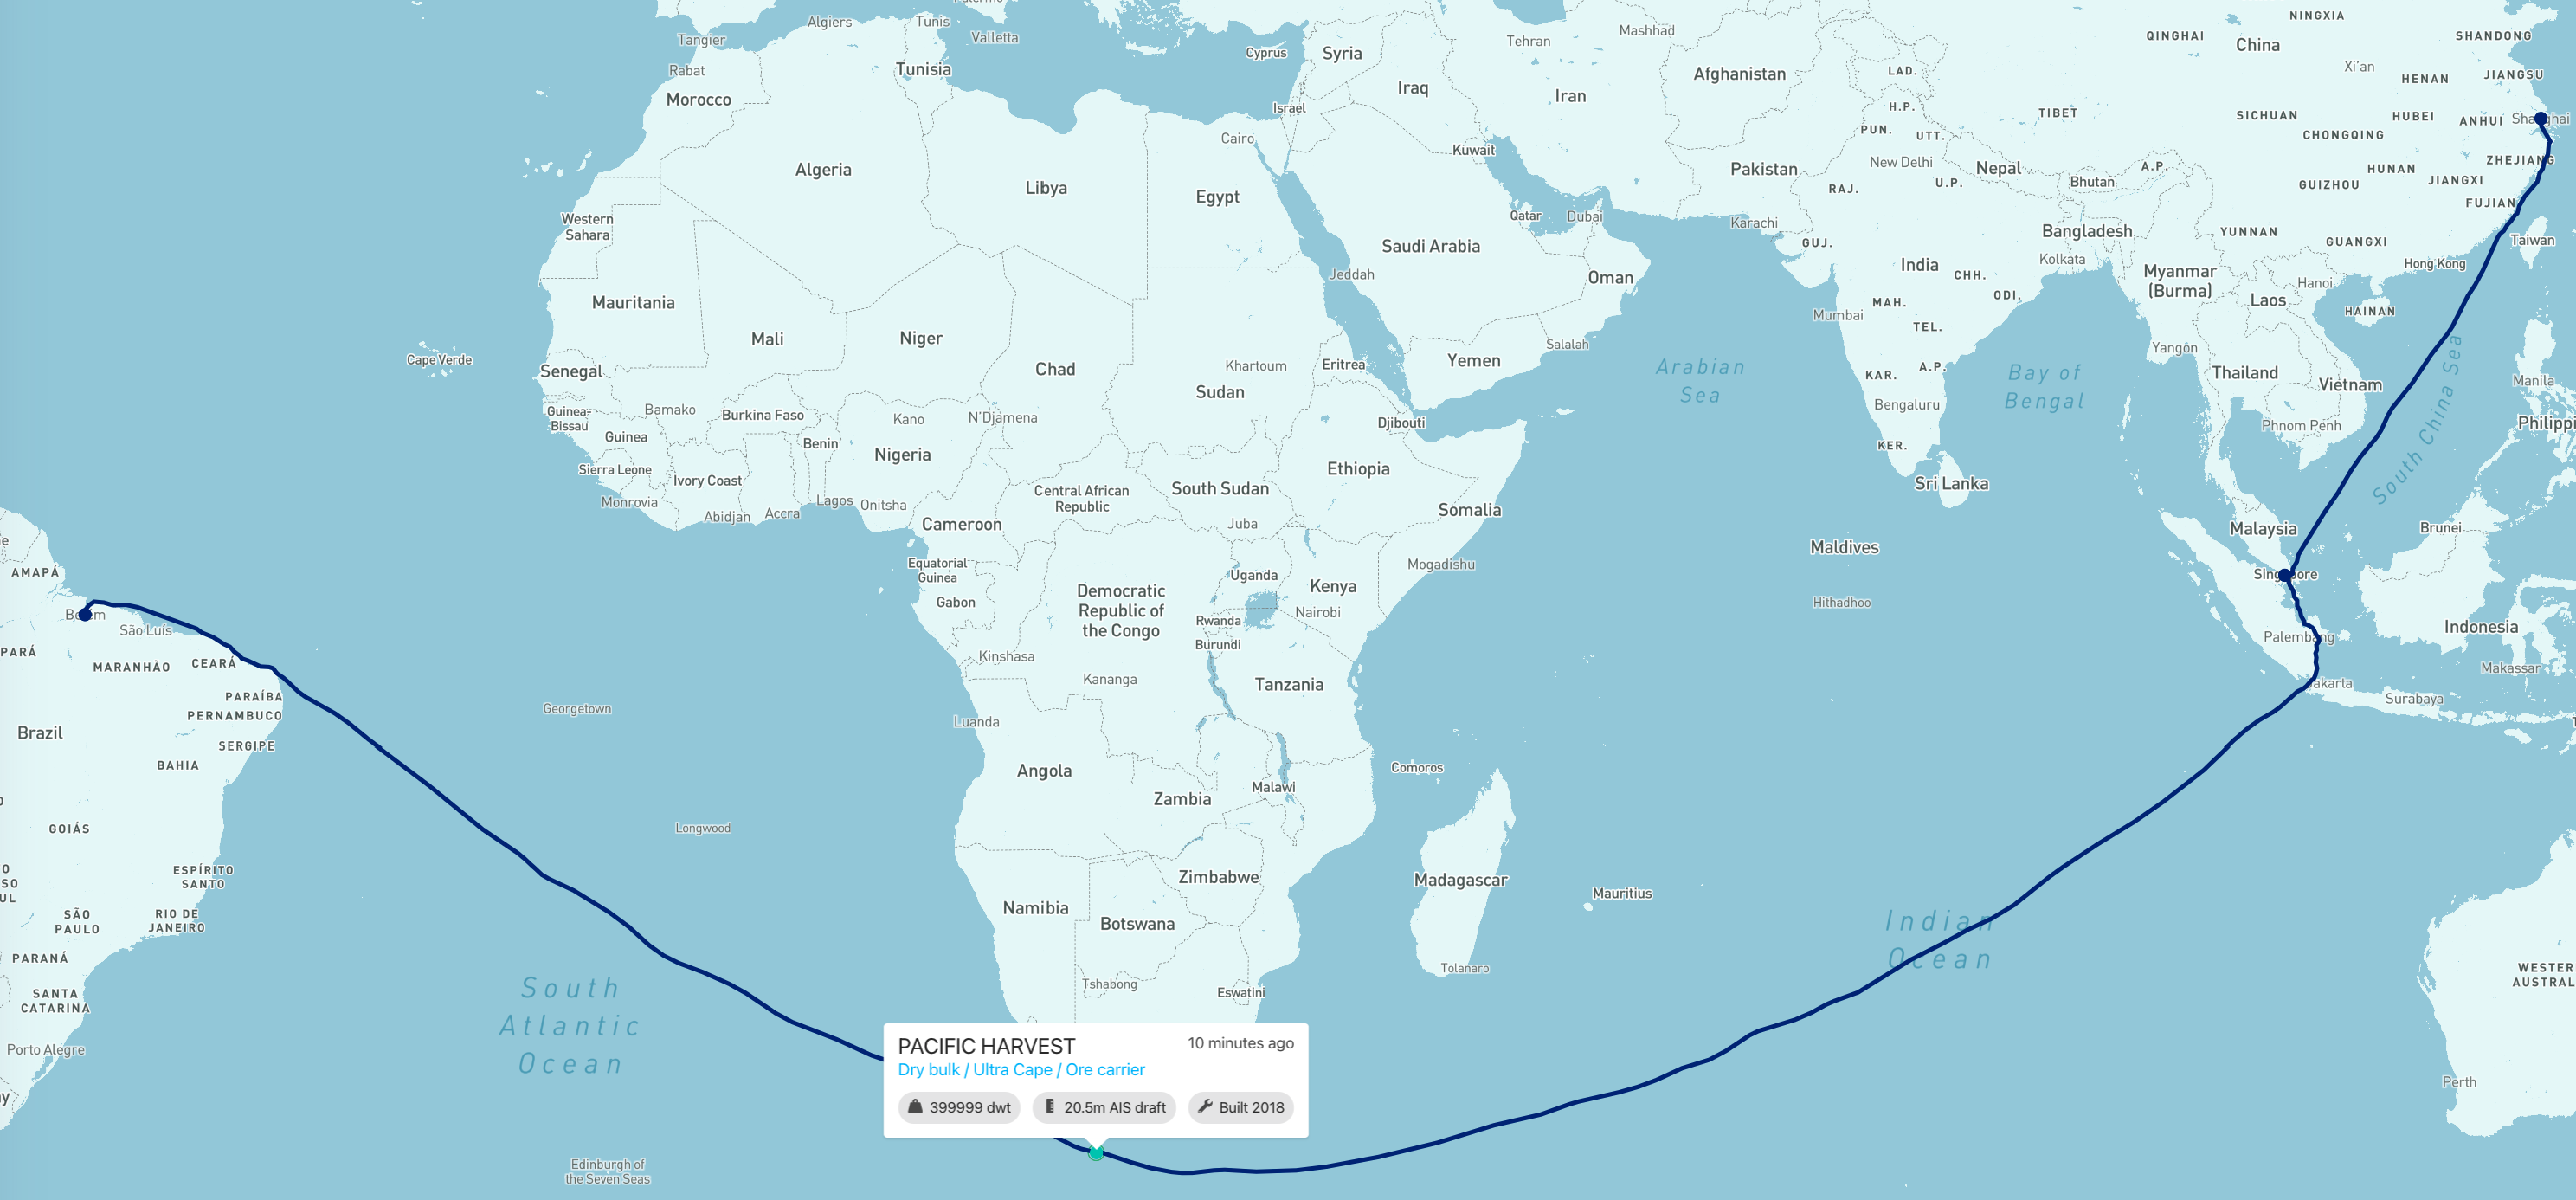
\includegraphics[width=0.9\textwidth]{figures/mo_voyage}
    \caption{Example voyage, created using \acrshort{mo}'s route planner tool, for a traveling vessel (Pacific Harvest), traveling from Brazil to China while stopping at Singapore to refuel.}
    \label{fig:example_voyage}
\end{figure}

To summarize, consider a voyage starting at Brazil and ending in Shanghai, China. Depending on the speed and fuel consumption of the traveling vessel, this voyage is around 12 000 nautical miles long and would take between 30 and 40 days. Thus, it is probable that a traveling vessel would stop to refuel at the bunkering port in Singapore. In this example (shown in \cref{fig:example_voyage}), one could either consider one complete voyage from Brazil to China, or one could consider two voyages; one going from Brazil to Singapore, and another going from Singapore to China. Assuming the vessel use the navigational status ``moored'' in Brazil and China only, the approach used in this thesis would consider one complete voyage from Brazil to Singapore, while a clustering-based method would consider the two shorter voyages.

\subsection{Trajectory similarity}

As will be further elaborated on in \cref{chap:related_work}, the current literature related to vessel destination predictions almost exclusively rely on some form of trajectory similarity. Therefore, trajectory similarity is also included in this thesis' proposed approach to vessel destination prediction. There are three main categories of trajectory similarity measurements: spatial, temporal, and tempo-spatial. Regarding vessel trajectories derived from \acrshort{ais}, they are not likely to share similar time intervals values as vessels travel at different speeds and at different times, therefore, for the purpose of this thesis, only spatial trajectory similarity measures are considered. This assumption is further corroborated by \cite{Zhang2020AISApproach} that arrived at a similar conclusion in their work developing a \acrfull{ml} -based approach to trajectory similarity measurements.

There are a number of spatial trajectory comparison methods that have been widely used for different purposes. The most relevant are the Hausdorff distance \parencite{magdy2015}, Fréchet distance \parencite{magdy2015}, and \acrfull{sspd} \parencite{besse2015review}. Out of these, the \acrshort{sspd} method is the most appropriate as it handles trajectories of different shapes and lengths well which is beneficial when comparing a trajectory from an ongoing vessel voyage to a set of complete historical ones. \cref{fig:sspd} shows an example from \cite{besse2015review} where two trajectories are compared and their symmetric distances are calculated.

\begin{figure}[htbp]  % order of priority: h here, t top, b bottom, p page
    \centering
    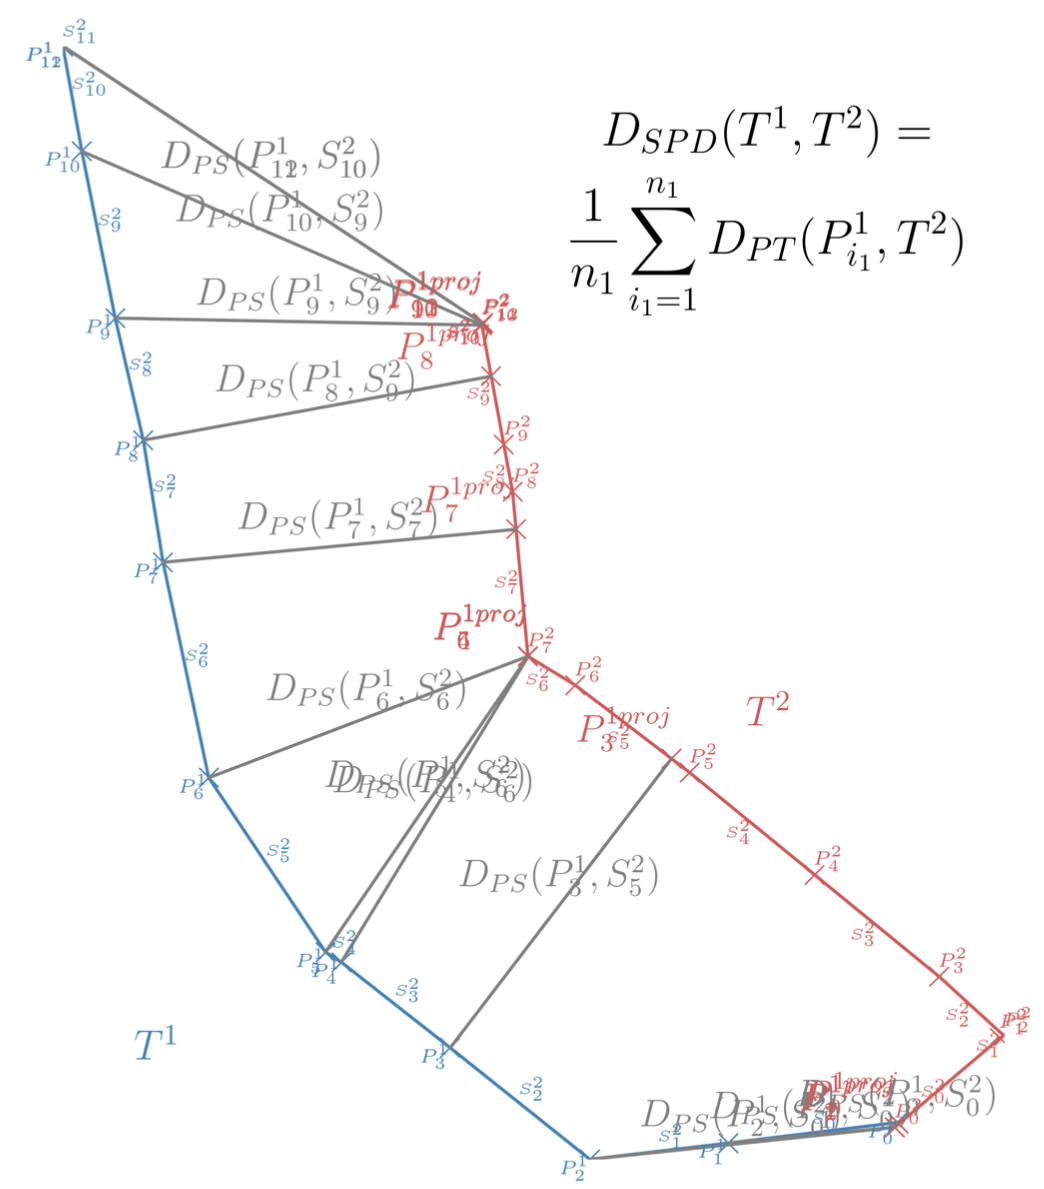
\includegraphics[width=0.5\textwidth]{figures/sspd}
    \caption{Segment Path Distance (SPD) in the SSPD process of comparing two different trajectories \parencite{besse2015review}}
    \label{fig:sspd}
\end{figure}

The methods mentioned thus far are all algorithmic approaches to measuring similarities between trajectories, however, there are also \acrshort{ml}-based methods as well such as the approach proposed in \cite{Zhang2020AISApproach} that also compares their results to the aforementioned methods. They used a \acrfull{rf} to measure similarities between a traveling trajectory and every historical trajectory traveling from the same departure port in order to predict the next destination port for a vessel. They achieved a higher general accuracy when compared to algorithmic methods such as \acrshort{sspd}. Moreover, for similar purposes, some unsupervised clustering methods have also been applied to similar problems such as the \acrfull{dbscan} which is capable of sequentially finding patterns in points and trajectories. This approach is more frequently used in trajectory predictions on a small geographical extent such as for collision detection and anomaly detection.

\subsection{Machine learning (ML)}

\begin{figure}[htbp]  % order of priority: h here, t top, b bottom, p page
    \centering
    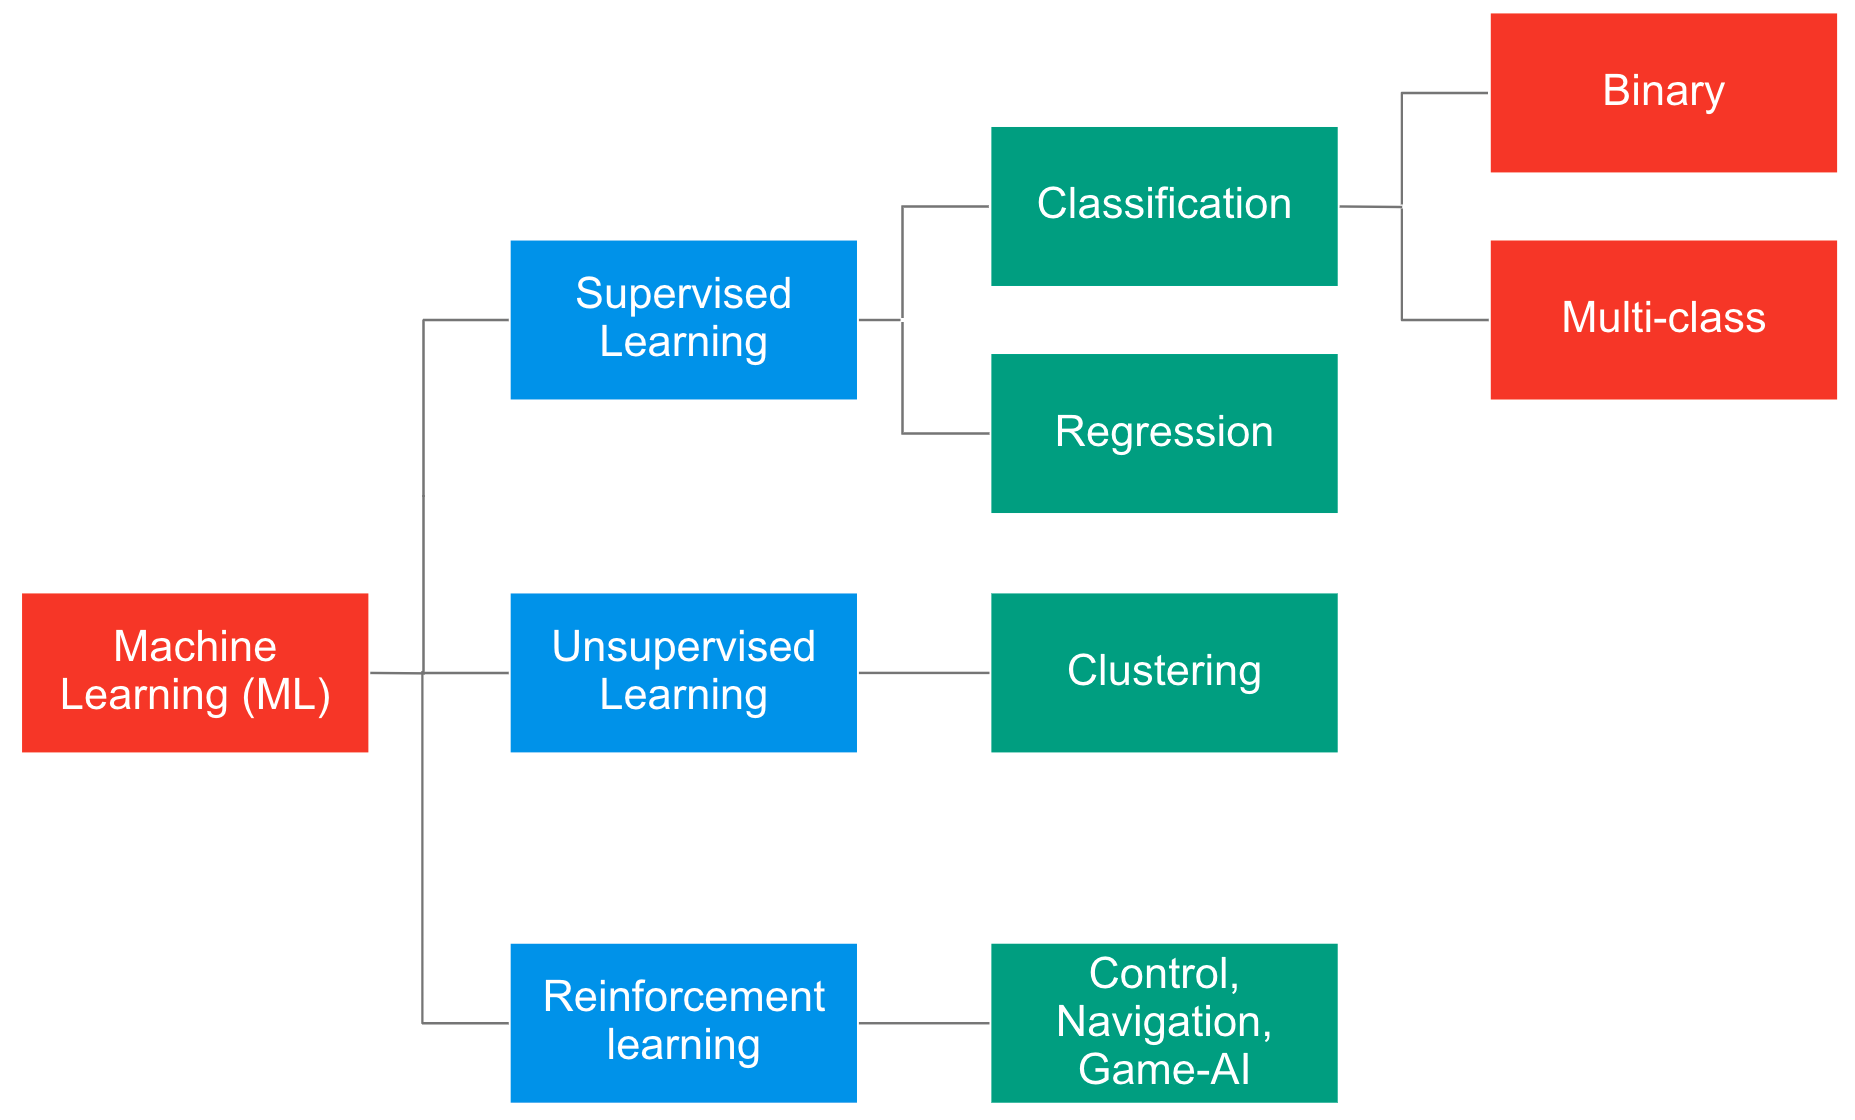
\includegraphics[width=0.75\textwidth]{figures/ml-terms}
    \caption{Machine Learning (ML) hierarchical terminology}
    \label{fig:ml_terms}
\end{figure}

\acrfull{ml} is an umbrella term describing computer algorithms that automatically adapt and improve based on experience. There is a vast number of different \acrshort{ml} algorithms applied to different problem areas. \acrshort{ml} is mainly divided into three broad categories: supervised learning, unsupervised learning, and reinforcement learning. In supervised learning, in the training process, both input and the desired output are provided to the model. The model finds patterns and correlations between input and output data during the training process, and when the model is trained or fitted, it is capable of guessing output given only input. In unsupervised learning, no output labels are provided to the model leaving the model to find patterns in the input set on its own. Clustering is an example of unsupervised learning as the model finds and labels patterns in input data without any external guidance. Reinforcement learning is a dynamic approach to \acrshort{ml} where the model continuously learns while trying to achieve a goal. In this method, the model navigates a problem space, and the program rewards or punishes the model that tries to optimize for rewards. In regards to topics covered by this thesis, \acrshort{ml}-based trajectory comparisons involve unsupervised learning, while predicting destination ports is supervised as the historical destinations are known.

\begin{figure}[htbp]  % order of priority: h here, t top, b bottom, p page
    \centering
    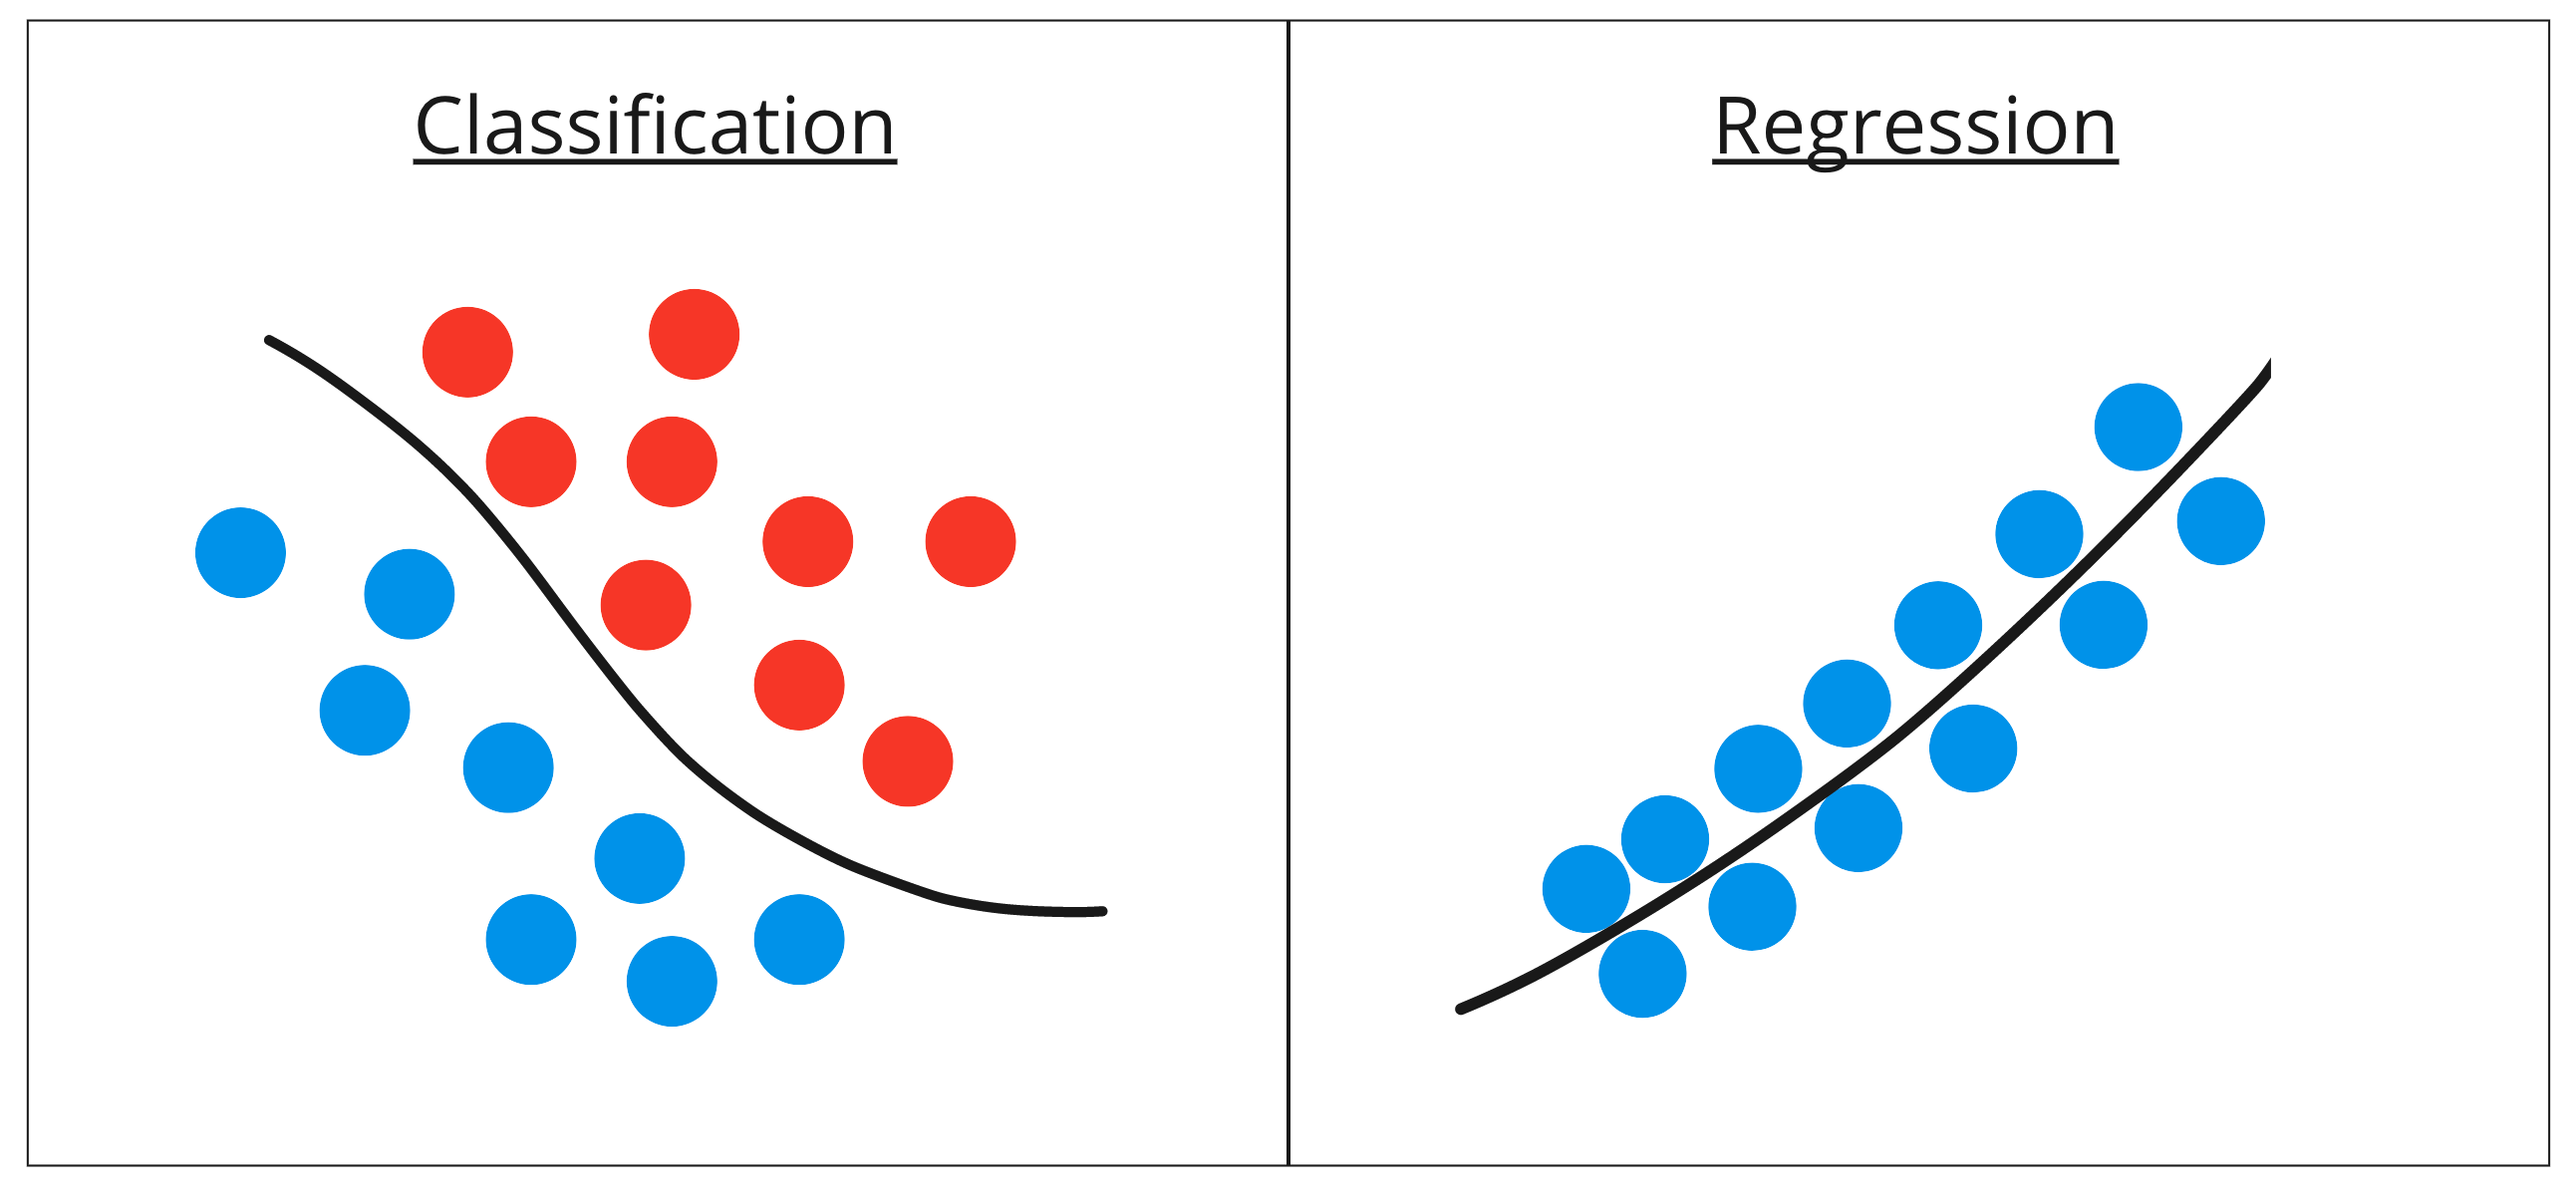
\includegraphics[width=0.75\textwidth]{figures/class_regg}
    \caption{Example showing the difference between classification and regression tasks}
    \label{fig:classification_regression}
\end{figure}

Moreover, supervised learning can further be divided into regression and classification problems. The main difference between the two is that classification aims at predicting a label, or a class, while regression predicts a quantity that is not necessarily present in the training data. For instance, a regression model can be used to predict the price of an item for sale, while classification can be used to label emails as "spam" or "not spam". \cref{fig:classification_regression} shows the difference between classification and regression. The example of classifying emails as ``spam'' or ``not spam'' would be considered a binary classification problem as there are only two possible labels, however, classification can also involve predicting more than two outcomes which is commonly referred to as multi-class classification. In the context of this thesis, predicting a vessel's destination port can be formulated as a multi-class classification problem as every possible destination port are different possible labels for a given voyage in progress. \cref{fig:ml_terms} shows the how \acrshort{ml} is hierarchically divided into more specific terms relevant for the scope of this thesis.

\begin{itemize}
    \item Cross-validation
    \item Hyperparameter optimization
\end{itemize}

\section{Technologies and protocols}

\subsection{Database system}

All the data that is used throughout this thesis for analysis is collected and stored in a \textit{PostGreSQL} database. \textit{PostGreSQL}, or \textit{Postgres}, is an open-source object-relational database management system that supports the extended subset of SQL standards. One major advantage of using \textit{Postgres} is the support for plugins such as \textit{PostGIS} that provides tools for dealing with \acrshort{gis} and geometric data. In this thesis, \textit{PostGIS} is frequently used to store and process geographical trajectory data for vessel voyages. Throughout this thesis, when referring to the proposed methodology and results, terms such as database, table, row, and column refers to the \textit{PostGreSQL} database used and its tables with rows, and columns.

\subsection{Programming languages and tools}

The main programming languages used throughout this thesis are Golang and Python. Golang is primarily used in constructing the initial data foundation which requires dealing with databases, trajectory building and validation. Golang is chosen for this because of its performance benefits and ease of use. For data analysis and machine learning, Python is the main programming language of choice. Most code provided to the reader in this document is written with the focus of readabilty over efficiency.

\subsection{Automatic Identification Systems (AIS) data}
\label{sec:ais_data}

\begin{figure}[htbp]  % order of priority: h here, t top, b bottom, p page
    \centering
    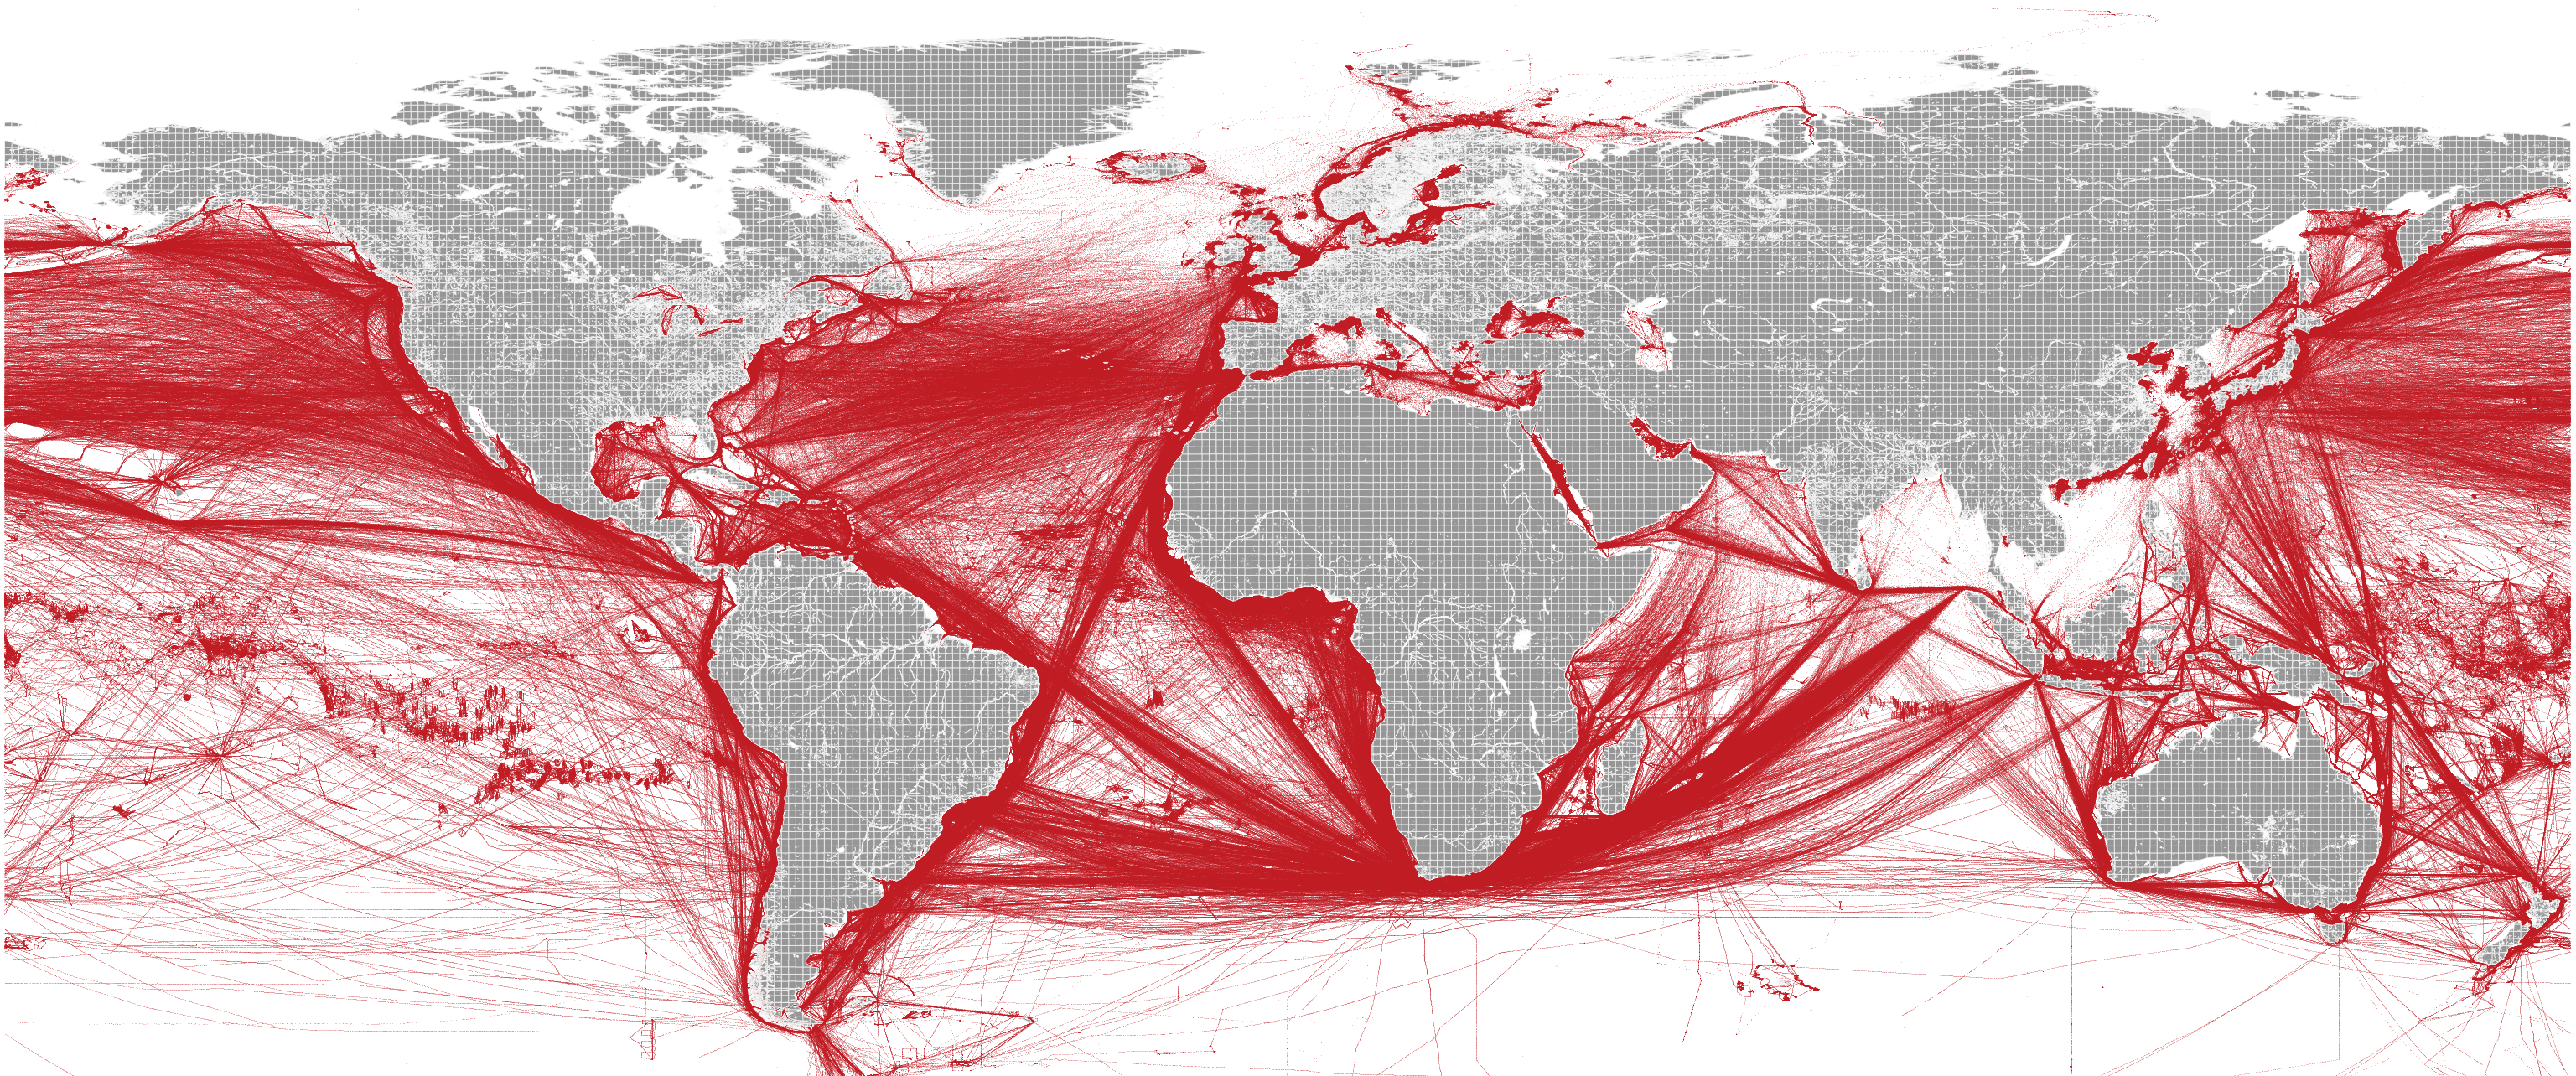
\includegraphics[width=1.0\textwidth]{figures/ais_history}
    \caption{Vessel positions derived from 100 million AIS positional reports}
    \label{fig:ais_positions}
\end{figure}

As already mentioned in \cref{sec:topics_covered}, \acrfull{ais} was initiated by \acrfull{imo} and since 2004 every commercial and passenger vessel exceeding 299 \acrfull{gt} is required to carry an \acrshort{ais} transmitter. These transmitters broadcasts \acrshort{ais} messages following the \gls{aivdm} protocol. The \gls{aivdm} protocol contains two main types of reports: positional and static. The positional reports contains automatically collected information such as the transmitting vessel's \acrfull{mmsi} number, the current timestamp, and the vessel's current navigational data including the current geographical coordinates, \acrfull{sog}, \acrfull{cog}, true heading, \acrfull{rot}, and more. The static reports contain additional information about the vessel and its current voyage, some of which are manually inputted, such as the vessel's \acrshort{imo} number, name, dimensions, draft, intended destination and \acrfull{eta}. As an example, \cref{fig:ais_positions} shows a visualization of 100 million \acrshort{ais} randomly chosen positional reports from a collection of historical \acrshort{ais} positions for global collection of shipping vessels. In relation, the historical \acrshort{ais} dataset used in this thesis consists of more than one billion records ranging from December 2019 to February 2021.

Regarding vessel identification in the \gls{aivdm} protocol, there are mainly two values that are unique to a given vessel: the \acrshort{mmsi} and \acrshort{imo} numbers. Either of these should be unique on their own for a given vessel, however, \acrshort{mmsi} numbers can be recycled under certain conditions such as when a vessel is put out of commission while the \acrshort{imo} number is specific to a vessel's hull. Therefore, \acrshort{imo} is the preferred identifier, however, since the \gls{aivdm} protocol divides these identifiers into positional and static reports, both need to be considered in order to use both static and positional \acrshort{ais} information.

\section{Initial data foundation}

This section describes the form and meaning of the data that forms the foundation of the thesis' proposed solution. The data is provided by the collaborative company \acrfull{mo} to the author.

\subsection{Vessel departure and arrival detection}
\label{sec:vessel_transitions}

\acrshort{mo} collects live \acrshort{ais} messages provided by a few sources, and in addition, they keep track of their navigational statuses as they are transmitted in the \gls{aivdm} protocol. These status attributes describe the current navigational state of the vessel for purposes of planning and security. Implicitly, these messages can indicate that a vessel has arrived or departed from a given port which can be used to detect voyages. When a vessel has concluded her journey and arrives at a port, the navigational status is changed to \textit{"MOORED"}, and when departing a port, the status is changed to \textit{"UNDERWAY USING ENGINE"} or \textit{"UNDERWAY SAILING"}. There are also other navigational statuses that could be relevant for voyage information such as \textit{"AT ANCHOR"} which could indicate that a vessel is bunkering (refueling) or is waiting for access to a berth that is congested. Currently, transitions from a status that indicates that a vessel is moving to the status \textit{"MOORED"}, and from \textit{"MOORED"} to moving are collected and labeled as arrivals and departures from or to the closest port within a given radius. This has proven to be a good method of identifying voyages and voyage trajectories between two ports as positions transmitted between a departure and arrival can be collected into a voyage trajectory that can be compared to other trajectories for analytical purposes. Throughout this thesis, this concept is referred to as vessel transitions.

\subsection{Additional vessel information and segmentation}
\label{sec:vessel_info_segments}

\acrshort{mo} has implemented a system for categorizing vessels into different segments, subsegments, and further variations. These segmentations are based on various factors such as the dimensional data provided by \acrshort{ais} messages as well as details provided by external vessel information sources and even user and manual input. The most important factors are the vessel type from the \gls{aivdm} protocol and the carry range, measured in \acrshort{dwt}, of the vessels which indicates how much cargo it can carry. This segmentation of vessels is highly relevant to voyage patterns as vessels of different types and sizes travel to different ports and countries for different shipping companies. This is further shown in \cref{fig:segment_map} which shows, from an image of \acrshort{mo}'s web platform, how different subsegments of the dry bulk cargo segment travels in different areas of the world. Since this categorization provides valuable insights into voyage patterns, vessel segmentation values are included in this thesis' proposed approach to vessel destination prediction.

\begin{figure}[htbp]  % order of priority: h here, t top, b bottom, p page
    \centering
    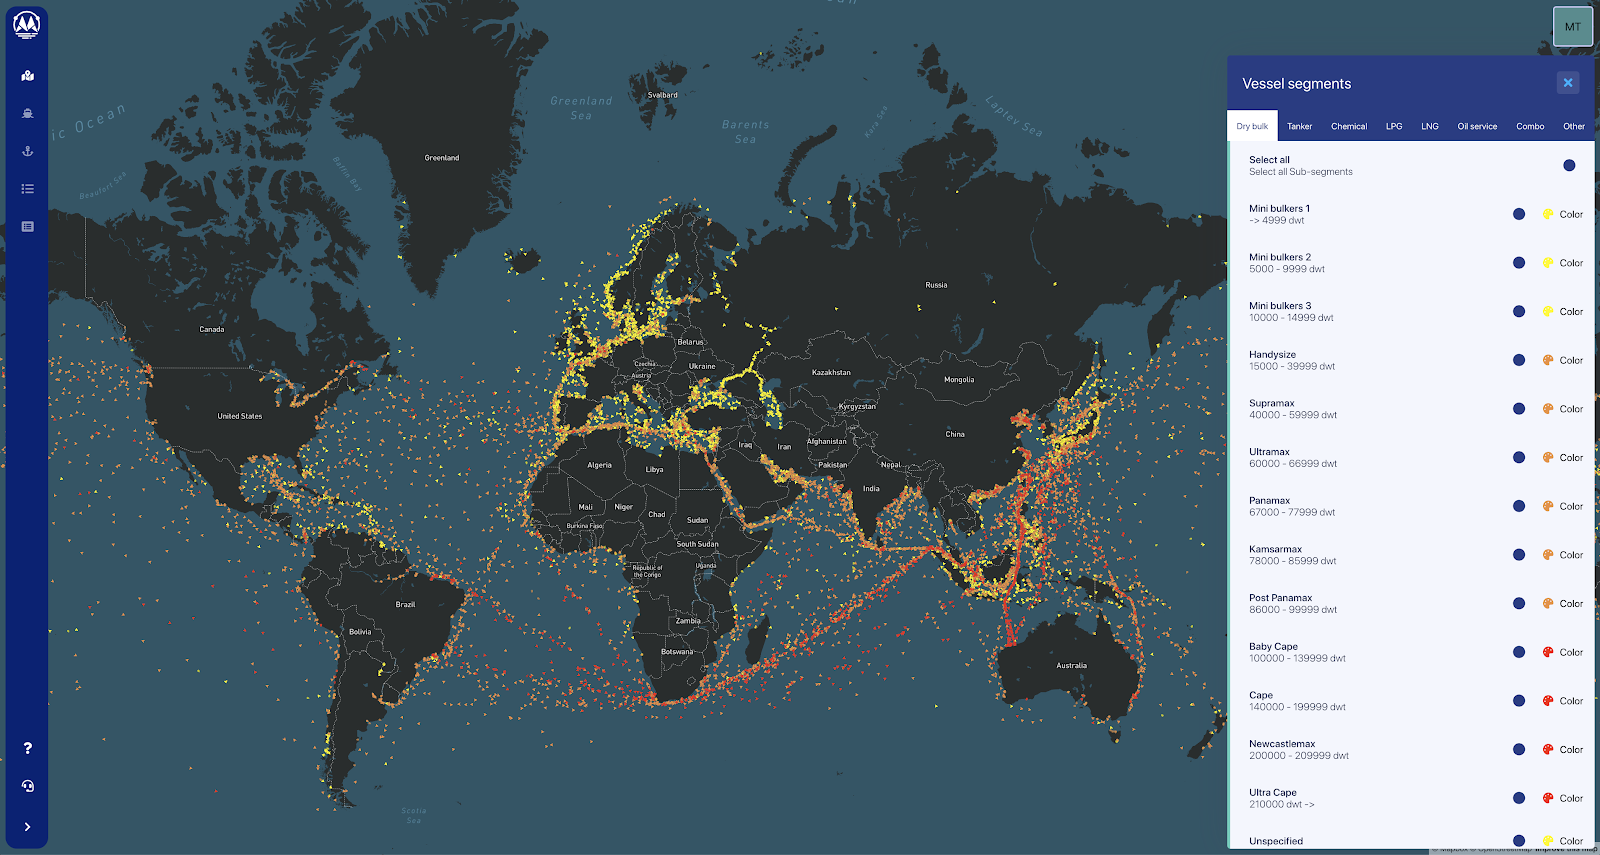
\includegraphics[width=1.0\textwidth]{figures/segment_map}
    \caption{\acrfull{mo}’s segmentation of vessels where yellow vessels are smaller than reds}
    \label{fig:segment_map}
\end{figure}

Moreover, \acrshort{mo} also has extensive vessel details for every vessel structured as a questionnaire in their product. This vast questionnaire contains information and fields from a combination of standards in the industry such as Q88\footnote{\url{https://corp.q88.com/}}. Data for the questionnaire is also collected from a number of external sources such as IHS Merkit\footnote{\url{https://ihsmarkit.com/index.html}} and DNV\footnote{\url{https://www.dnv.com/}}. Users of \acrshort{mo} also have the possibility of suggesting changes to a public version of this questionnaire for any vessel. These changes are verified by \acrshort{mo} and published if the information proves accurate. This detailed description of vessels provides creates a big potential for data analysis and a potential \acrshort{ml} model that is highly aware of specific vessels which ultimately may affect its traveling patterns. However, in this thesis, the main focus is on the vessel segmentation when developing the proposed solution. This data is later referred to as vessel segments and includes both the vessels' segment and sub-segment.

\subsection{Shipping ports}
\label{sec:shipping_ports}

\acrshort{mo} has an extensive port database containing more than 5600 ports. From sources such as UNECE it is possible to find a vast number of ports, however, only a sub-set of the worlds known ports are used by \acrshort{mo} as these are considered relevant shipping ports. The process of determining what ports are relevant shipping ports is a continuous manual process in \acrshort{mo} but it ensures that the available selection of ports is highly relevant for the industry. Furthermore, all ports are identified by their \gls{locode}. This is a five-letter unique identifier provided and managed by the United Nations (UN). In the five-letter code, the first two indicate the port's country of origin, while the three last indicate a more specific location within the origin country. As an example, the \gls{locode} for the port of Oslo is \texttt{NOOSL} where ``NO'' stands for Norway, and ``OSL'' stands for Oslo. For comparison, a similar system is used for international airports. For this thesis, only the 5600 relevant ports are considered for the analysis.

\chapter{Related work}

The topic of \acrfull{ais} -based predictions has already been explored quite extensively, especially in recent years as \acrshort{ais} systems has become an enforced standard for commercial vessels in the industry. However, the \acrshort{ais} standard has mainly been standardized for the purpose of maritime safety and navigation, and the existing academic work on this topic reflects this. Therefore, most of the related work consists of vessel trajectory predictions for the purpose of foreseeing a future collision situation or for detecting anomalies from detected shipping lanes. These types of predictions are applicable for predicting a vessel's future position in a short time interval, in a smaller geographical scale, but with high positional accuracy.

In order to establish the current state of the art of the topic area and establish to what extent the literature answers the proposed research questions, a literature review was conducted which is explained in this section.

\section{Literature review}
\label{sec:lit_review}

As already mentioned, based on initial research into the thesis' topic area, there seemed to be an apparent trend in motivations of related work directed at short-term predictions for safety and navigational purposes. In contrast, this thesis aims at using \acrshort{ais}, and other attributes, for longer term predictions, or more accurately, port destination predictions. However, because of the exploratory nature of thesis, the literature review conducted was broad in order to include work that might have taken a different approach to solve the same problem. In order to organize the resulting papers, a categorical separation of papers based on motivation was defined as follows:

\begin{enumerate}
\setcounter{enumi}{-1}
    \item The paper's motivation deems it completely irrelevant to the topic area.
    \item The paper's motivation includes vessel predictions, but on a smaller time or geographical scale making it irrelevant for comparison.
    \item The paper's motivation includes destination predictions making it relevant enough for further analysis.
\end{enumerate}

\textit{Category 0} is defined to filter out papers that were irrelevant but could not be excluded by narrowing the search query. \textit{Category 1} includes paper that relates to the established trend mentioned earlier where the proposed method seems relevant on a small scale, but is ultimately not applicable to the thesis' problem area. It also includes papers that considers relevant topics but not relevant solutions. Finally, the papers labeled with relevancy \texttt{2} falls within \textit{Category 2} and includes papers that falls within the same topic area and are relevant for further analysis in regards to the research questions.

In order to determine what papers fitted \textit{category 1} and \textit{2}, papers with a relevance higher than zero were further analyzed in order to determine the following attributes:

\begin{itemize}
    \item Motivation and goals
    \item Data source
    \item Prediction method
    \item Geographical extent
    \item Time interval
    \item Validation method
    \item Validation, or performance metrics
\end{itemize}

In this literature review, the primary search engine used was \textit{Scopus}\footnote{\url{https://www.scopus.com/}} as it seemed to return the best search results without an excess of less relevant papers that was returned by other search engines such as \textit{ScienceDirect}\footnote{\url{https://sciencedirect.com}} and \textit{Google Scholar}\footnote{\url{https://scholar.google.com}}. Furthermore, the chosen search query was also ran on the \acrshort{ntnu} university library \textit{Oria}\footnote{\url{http://ntnu.oria.no/}} in order to find overlap and additional results not found by \textit{Scopus}.

\subsubsection{Search query and filters}

The objective of the literature review was to conduct a broad search detecting papers related to multiple relevant topics such as \textit{vessel destination prediction}, \textit{vessel trajectory prediction}, \textit{vessel availability forecasting}, and \textit{maritime logistics}. Therefore, the search query used in the literature review was designed to find papers within multiple topics and was derived at from testing multiple queries on multiple search engines.

For instance, the following queries were tested using the search engine provided by \textit{ScienceDirect}:

\begin{itemize}
    \item `vessel trajectory' OR `ship trajectory' resulted in \textbf{421} papers
    \item ais AND (`vessel trajectory' OR `ship trajectory') resulted in \textbf{150} papers
    \item ais AND (prediction OR predicting) AND (`vessel trajectory' OR `ship trajectory') resulted in \textbf{108} papers
\end{itemize}

The above queries returned a large number of papers relevant to \textit{category 1}, so in order to find more relevant papers, more specific queries were also tested:

\begin{itemize}
    \item `vessel destination' OR `ship destination' OR `vessel availability' resulted in \textbf{389} papers
    \item ais AND (`vessel destination' OR `vessel availability') resulted in \textbf{25} papers.
    \item ais AND (predicting OR forecasting) AND (`vessel destination' OR `vessel availability' OR `ship supply') resulted in \textbf{18} papers.
\end{itemize}

The search terms that seemed to return the most relevant papers was combined into the final query used in the literature review shown in \cref{lst:search_query}.

\begin{lstlisting}[
    caption={Search query used in literature review},
    label=lst:search_query
]
ais AND (
    predict OR predicting OR forecast OR forecasting
) AND (
    vessel OR ship OR maritime
) AND (
    destination OR availability OR supply OR trajectory OR logistics
)
\end{lstlisting}

Moreover, the following filters was used to limit the search result:

\begin{itemize}
    \item The paper must be published in the last 5 years.
    \item The paper must be available in English.
    \item The paper must be available using the access rights provided by \acrshort{ntnu}.
\end{itemize}

As already mentioned, the search query was ran on the search engine \textit{Scopus}, thus the search query and filters was modified to the search engine's format as shown in \cref{lst:search_query_scopus}.

\begin{lstlisting}[
    caption={Search query used in Scopus including filters},
    label=lst:search_query_scopus
]
TITLE-ABS-KEY (
    ais AND (
        prediction OR predicting OR forecast OR forecasting
    ) AND (
        vessel OR ship OR maritime
    ) AND (
        destination OR availability OR supply OR trajectory OR logistics
    )
) AND PUBYEAR > 2014 AND (
    LIMIT-TO ( DOCTYPE , "cp" ) OR
    LIMIT-TO ( DOCTYPE , "ar" ) OR
    LIMIT-TO ( DOCTYPE , "re" ) OR
    LIMIT-TO ( DOCTYPE , "ch" ) OR
    LIMIT-TO ( DOCTYPE , "Undefined" )
) AND ( EXCLUDE ( SUBJAREA , "MEDI" ) )
\end{lstlisting}

\subsubsection{Results}

The defined search query returned a total of \textbf{80} papers from the \textit{Scopus} search library and \textbf{22} from \textit{Oria} where out of which \textbf{7} papers did not overlap with results from \textit{Scopus}. These \textbf{87} papers formed the basis of the literature review.

The papers were evaluated based on the level of relevance as defined in \cref{sec:lit_review}. Out of the \textbf{80} papers, \textbf{49} fell within \textit{category 0}, \textbf{32} within \textit{category 1}, and \textbf{6} within \textit{category 2}.

The large number of irrelevant papers resulted from the broadness of the query that was designed to find results in multiple topic areas. Furthermore, there were some papers that was medical in nature but not labeled correctly in \textit{Scopus} and was returned as the term \acrshort{ais} is also an acronym of \textit{Arterial Ischemic Stroke}. Some papers were also not publicly available but was not excluded by the search, while other papers were deemed irrelevant as they concerned topics such as mapping fishing areas in a specific region, power and performance predictions using \acrshort{ais} data, or high level discussions of potential applications of \acrshort{ais} data analysis.

The large number of papers within \textit{category 1} further confirms the general trend of \acrshort{ais} -based predictions as the primary goal of most of the resulting papers were to predict future positions of vessels within a shorter time intervals for the purpose of either safety and navigation or anomaly detection. None of the papers within \textit{category 1} seemed applicable to predict vessel destination ports at a global scale, however, for reproducibility, all papers with a relevancy of \textit{1} are listed in \todo{APPENDIX}.

% most relevant papers collected from literature review
\begin{table}[tbp]
    \centering
    \csvreader[
      tabular=p{0.55in} p{1.7in} p{1.6in} p{0.7in} p{0.3in},
      table head=\hline \bfseries{Paper} & \bfseries{Goal} & \bfseries{Pred. method} & \bfseries{Geo-extent} & \bfseries{Time},
      before line=\\\hline,
      late after last line=\\\hline % horizontal line at the end of the table
    ]{
        csvtables/most_relevant.csv
    }{}{\csvlinetotablerow}
\caption{Papers collected from literature review with relevant geographical and time limitations}\label{tab:most_relevant_papers}
\end{table}

The remaining \textbf{}6 papers (listed in \cref{tab:most_relevant_papers}) were deemed relevant enough to further analyze in order to answer the research questions defined in \cref{sec:research_questions}. In addition, \cite{lechtenberg2019}, which was discovered during the process of testing queries, was also included in the analysis as it seemed highly relevant toward availability forecasting, but did not appear when using the two search engines in the final review.


\todo{copied from RPP}
\paragraphheader{RQ 1: What prediction methods can be used to predict vessel availability?}

\cite{lechtenberg2019} used a combination of several prediction methods in order to predict vessels’ next destination region, estimated time of arrival (ETA), and anchor time (AT) within regions. For predicting the next destination region the \textit{Markov Decision Process} was used as there are a limited number of possible regions (44) that a vessel can travel to. For the ETA and AT predictions, an \textit{XGBoost} method was applied. However, the extent of the regions was not disclosed, and although it was explained that port frequencies were used to determine regional availability, the accuracy of port frequencies was also not disclosed.

\paragraphheader{RQ 2: What prediction methods can be used to predict vessel destinations?}

\cite{ZHANG2020102729} was the second paper found which fitted within \textit{category 1}, and used a random forest approach to compare a given vessel’s current trajectory with all historical trajectories from the same departure port. They also used port frequency to normalize the results. In this way, they managed to achieve good results by combining both methods for predicting port destinations as well as city destinations. This method was unique as it considers multiple aspects of vessel voyages compared to the other methods.\\

\paragraphheader{RQ 2A: What type of data did they rely on?}

All of the aforementioned methods relied on historical AIS data collected by a combination of satellite and land-based base stations. \cite{ZHANG2020102729} also relied on an extensive port data base consisting of over \textbf{10 000} ports.

\paragraphheader{RQ 2B: How much depth of the data was relevant to the results?}

\cite{ZHANG2020102729} exclusively relied on the navigational data supplied by the AIS protocol. The navigational part of the AIS protocol includes coordinates, speed over ground (SOG), rate of turn (ROT), course over ground (COG), and more. Furthermore, \cite{ZHANG2020102729} also considered port frequencies, however, this frequency is deducted from the navigational part of the AIS data. Similarly, \cite{lechtenberg2019} also used port frequencies to predict regional availability, ETA, and AT. As already mentioned in \cref{sec:problem_desc}, destination and ETA values are included in the AIS protocol, however, as they are manually inputted by crew members they are not accurate. This is reflected in the existing literature as none of the aforementioned methods takes these values into consideration. Thus, it seems that all the relevant research ultimately only considers the navigational part of the AIS protocol for future predictions.

\paragraphheader{RQ 2C: How successful were they at predicting vessel destinations?}

\cite{lechtenberg2019} claims a \textit{98\%} accuracy when it comes to predicting a vessel’s next region, however, this value is presumed to vary depending on the size of the regions which is not disclosed in the paper. \cite{ZHANG2020102729} claims to have achieved a \textit{66.57\%} accuracy level for port-based predictions and \textit{81.65\%} accuracy for city-based predictions. As there is very little research that directly concerns predicting port or region destinations it is hard to establish a general accuracy of the state of the art. The closest assumption would be around \textit{70\%} for port predictions and \textit{98\%} for region predictions.

\paragraphheader{RQ 2D: How applicable were they toward predicting vessel availability?}

\cite{lechtenberg2019} was directly applicable and applied toward predicting vessel availability with a global set of regions. \cite{ZHANG2020102729} was not directly applied to forecast availability although it shows a very promising and generic method of predicting vessel’s future destinations unrestricted from time intervals or geographical areas. It is therefore very applicable toward predicting availability if applied to a global set of vessels. The rest of the aforementioned papers does not seem applicable toward availability if not combined with other methods that enable them to give accurate predictions globally.

\paragraphheader{RQ 3: How can the quality of the prediction methods be ensured?}

\cite{lechtenberg2019} does not go very in-depth on this topic, however, the paper mentions dividing the data into \textit{90\%} training data and \textit{10\%} test data. The accuracy metric is taken from how much of the test data was accurate. \cite{ZHANG2020102729} did an extensive evaluation of their method including the five-folder cross-validation method to ensure the model is not over-fitted. This process includes dividing the data into five “folders” and using one folder at a time for evaluation and the others for training. If the general accuracy does not vary much across the evaluation folders, the model is not overfitted.

\paragraphheader{RQ 3A: What metrics, or measurements, are used to establish quality?}

It seems that accuracy is the main measurement used to establish quality. Furthermore, \cite{lechtenberg2019} mentions using both the “mean absolute error” (MAE) and the “root mean square error” (RMSE) as quality indicators. \cite{ZHANG2020102729} mainly uses “average prediction distance error” (APDE) as their quality indicator which is based on the distance between the predicted trajectory and the actual trajectory.

\paragraphheader{RQ 4: How extensive is the impact of considering segmentation for prediction methods?}

None of the papers found within the research areas considers any type of segmentation of vessels. It is, therefore, impossible to answer this research question based on the current state of the art of the problem area.


\begin{sidewaystable}
    \centering
    {\small
    \begin{tabular}{|l|l|l|l|l|l|l|}
    \hline
        Paper & Motivation & Prediction method & Geographical scale & Time scale & Validation method & Validation metrics \\ \hline
        \cite{Alizadeh2020PredictionTrajectory} & trajectory similarity measurement for prediction of positions at time intervals & "spatial distance, bi-directional distance, speed distance" & "region (strait of georgia, USA)" & "10, 20, 30 minutes" & "sorenson similarity index (SSI), case study in region" & accuracy \\ \hline
        \cite{Alizadeh2021VesselData} & Vessel trajectory prediction for collision avoidance & "LSTM (RNN) with trajectory distance similarity measurements (TSSP, PSSP, TSSPL)" & "Strait of Georgia, USA" & Short term (10 - 40 mins) & 1 to 8 division of training and validation set & haversine distance accuracy (0.8 km to 3.5 km from 10-40 mins) \\ \hline
        \cite{Borkowski2017TheFusion} & data fusion prediction for collision avoidance integrated in navigation system & "ANN, data fusion, GRNN" & small (collision avoidance) & small & integrated and tested in real naviagtional system & RMSE \\ \hline
        \cite{Brandt2017MovingPrediction} & short time predictions of moving objects & "moving object data stream mangement systems, kNN " & "small, region in US" & small (10 minutes) & test cases & not explained \\ \hline
        \cite{Burger2020DiscretePrediction} & trajectory predictions for filling in gaps in AIS data & "DKF (discrete kalman filters), LRM" & small & small & single cases analysis on a vessel comparing two models & MED (mean euclidea distance) \\ \hline
        \cite{Chen2020ThePrediction} & cluster reconstruction not requiring training phase for short time frames & NPC clustering finding best possible next points & small & small & extensive comparisons with other methods & "accuracy, distance error" \\ \hline
        \cite{Dalsnes2018ThePrediction} & collision detection for autonomous vessels & NCDM & small (collision detection) & small (collision detection) & 90/10 training validation sets & RMSE \\ \hline
        \cite{Dijt2020TrajectoryShips} & collision avoidance for autonomous ships & sequence to sequence neural network & small (collision avoidance) & small (collision avoidance) & "90/10 data split of six hours trajectories, cross folder validation" & "absolute trajectory error, RMSE, MAE" \\ \hline
        \cite{DIng2020ALSTM} & longer time and multidimensional trajectory predictions & LSTM & small & 5-20 minutes & "training, validation, test set (8:1:1)" & MSE \\ \hline
        \cite{Forti2020PredictionNetworks} & sequence-to-sequence RNN approach & RNN with LSTM encoder-decoder architecture & region & small & 5-fold cross validation & RMSE \\ \hline
        \cite{Guo2018TrajectoryChain} & trajectory predictions MDTN (mobile delay tolerant network) & k-order multivariate markov chain & region (grid based) & small & "simulation, experiments" & accuracy \\ \hline
        \cite{Hexeberg2017AIS-basedPrediction} & collision detection & single neighbor search (SPNS) & region (trondheim) & small (10 minutes) & "training, validation sets, manually selected scenarios, validate with real trajectory" & RMSE \\ \hline
        \cite{Jin2020MaritimeNetwork} & longer range predictions for security motivations & "RNN, LSTM" & regional/small & small & model simulation & "distance accuracy over time, MAE, SSE" \\ \hline
        \cite{Kim2018PreprocessingArea} & predictions for Vessel Traffic Service (VTS) & NN & small & small & case study on region & speed and distance error \\ \hline
        \cite{Li2018ShipMining} & ceaner data extraction and mining for predictions & RBF neural network model & small (tested on river in china) & small-medium (hours) & simulation/case study on river in china & trajectory difference from real to simulated \\ \hline
        \cite{Li2019Long-termData} & longer term predictions for collision avoidance & "LSTM, longest comomon subsequence(LCS) algorithm, DBSCAN clustering" & small / collision avoidance & small / collision avoidance (15 min) & "applied to 4 regions, case studies" & distance error \\ \hline
        \cite{Lian2019ResearchAlgorithm} & "investigating particle filtering, near prediction, least squares estimation approach to predictions for smaller scale predictions" & "linear prediction, least squares, particle filtering" & small / collision avoidance & small / collision avoidance & "simulation, 9 hours of data" & "distance error, speed error" \\ \hline
        \cite{Liu2019VesselACDE-SVR} & trajectory prediction that also handles real time at sea & "SVR, ACDE, RNN" & small / collision avoidance & small / collision avoidance & training/validation sets & distance error \\ \hline
        \cite{Liu2020PredictingLearning} & "predicting trajectories for ship management, interpolating method for filling in missing AIS in trajectory" & "LSS-VM (least-squares support-vector machines) for predictions, cubic spline function to regulate trajectories via interpolation" & "independent of regions, but on a small scale (predicting distance not arrival ports)" & small (predicting next positions in trajectory) & four random trajectories selected for predictions & accuracy in distance/meters from actual trajectory \\ \hline
        \cite{Mao2018AnMining} & database for trajectory prediciton and mining & "interpolating trajectory reconstruction, are of interest bsed grid search, ELM and SLFN for predictions" & region based & medium (20 - 40 minutes) & original vs predicted trajectory & distance error \\ \hline
        \cite{Murray2018AOperations} & collision detection for autonomous vessels & Single point neighboir search method & small (collision detection) & 5-30 minutes & 90/10 training validation sets & RMSE \\ \hline
        \cite{Murray2019AnVessels} & collision avoidance & "gaussian mixture modelling, principle component analysis" & small / collision avoidance & small / collision avoidance & running 100 times randomly selecting points & distance error \\ \hline
        \cite{Murray2020AData} & trajectory predictions for early warnings and safety & "GMM clustering (gaussian mixture model), novel dual autoencoder" & region (tromsø) & 30 minutes (1 year or historical AIS) & distributed accuracy over time in the future (predicted positions vs actual positions) & accuracy at time intervals \\ \hline
        \cite{Rong2019ShipModel} & modelling uncertainty of trajectory predictions & "Bayesion model, Gaussian Process" & small / collision avoidance & "small / collision avoidance (10, 20, 30)" & "case study in region, training / validation data" & "accuracy, distance error" \\ \hline
        \cite{Suo2020ANetwork} & trajectory predictions for early warnings and safety & "GRU (gate recurrent unit), DBSCAN, comp. with LSTM" & tested on single port in china & "small, minutes to hour" & "training, validation, test set (not defined how much)" & accuracy \\ \hline
        \cite{Tafa2019AutomaticPrediction} & synthetic route representation and predictions & "DBSCAN, route similarity probability model" & east china sea region & 10-80 minutes & simulation & accuracy \\ \hline
        \cite{Tang2019ANetwork} & collision avoidance for automonous ships & LSTM & region in china & uses 10 min of data to predict 20 next minutes & training/validation sets & "MAE, MSE" \\ \hline
        \cite{Uney2019DataModels} & forecasting trajectories from historical and streaming trajectories & directed grid based bayesion model / gaussian mixture forecast density & tested on region (15x15 grid) & any (tested with 2 months of data) & real life case study in region & not explained \\ \hline
        \cite{Virjonen2018ShipMethod} & predictions in area in finnland that has to be several hours ahead in time & k-nearest neighbours & medium (region of finnland test case) & "medium, several hours" & nested leave-one-out-cross-validation (LOOCV) & distance accuracy \\ \hline
        \cite{Wang2020VesselGRU} & predicting vessel berthing trajectory for safety and collision avoidance & "Bi-GRU (tensorflow, keras)" & single port in china & small (minutes) & "training, validation set (not defined ratio), compared to other models" & MSE \\ \hline
        \cite{Xiao2020BigTechniques} & "for collision avoidance, better quering, more effective predictions" & "knowledge based particle filtering (PF), MLNN" & "smaller, limited to collision avoidance" & 3-10 minutes & testing different scnarios i.e. case studies & "sog, coc, and distance error" \\ \hline
        \cite{You2020ST-Seq2Seq:Prediction} & sequence-to-sequence RNN approach & "seq2se1 GRU, RNN, encoder/decoder" & "small, limited to 10m trajectories" & 10 minutes & "analysis in region (few rivers in china), training/validation set" & "AdaGrad, RMSProp" \\ \hline
        \cite{Zheng2020HeterogenousModeling} & combining multiple datasources like GPS and ARPA with AIS to improve predictions for safety & LSTM (on different data and a fusion component to merge the predictions) & small & small & "training, validation (1:10), and compare to other model" & MSE \\ \hline
        \cite{Zhou2019ShipNetwork} & collision avoidance in busy areas & back propagation nerual network & region (area in china) & small & training/validation 70/30 & RMSE \\ \hline
    \end{tabular}
    }
\end{sidewaystable}
\chapter{Feasibility study}

As already mentioned, the main motivation behind the thesis is derived from the observation that the existing methods of vessel destination prediction neglect data depth in their models. Especially, not considering the type and dimensions of vessels is presumed to be a major limitation of the existing literature. In order to establish this in an empirical manner, a feasibility study was conducted on the aspect of \acrfull{mo}'s novel segmentation of vessels. As part of the course work for the prior \acrshort{ntnu} course called \textit{“IMT4894 Advanced Project Work”}, such a feasibility study was  conducted to estimate the impact of vessel segmentation on the aspect of port frequencies. Port frequencies, or patterns of port arrivals and departures should reflect the fact that different vessels of different types travel in different patterns. Thus, if it is possible to show that segmentations have a significant impact on these patterns through port frequencies, it can be concluded that it will have an impact on vessel destination predictions.

The dataset used in this feasibility study mainly consisted of vessel transitions (as described in \cref{sec:vessel_transitions}), and port data (as described in \cref{sec:port_data}). The dataset also includes the vessel's segment and sub-segment (as described in \cref{sec:vessel_segments}). For a given port, every visiting vessel was assigned the attribute \textit{NextPort} that indicated the next arrival port after departing the given port. \cref{fig:apw_dataset} shows an example of vessels arriving at the port of Oslo (\texttt{NOOSL}).

\begin{figure}[htbp]
    \centering
    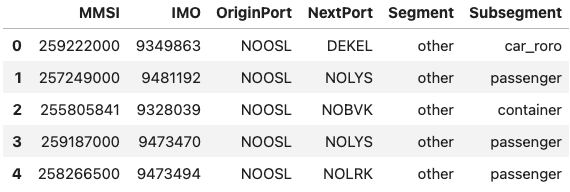
\includegraphics[width=.8\textwidth]{figures/apw/apw_dataset.png}
    \caption{A sample of the dataset used in the feasibility study}
    \label{fig:apw_dataset}
\end{figure}

In the feasibility study, there were two main steps in the analysis process. Firstly, a single-case analysis was conducted on a port known to the author to establish a more thorough overview of the traveling patterns of different vessel types and to gain an understanding of how to interpret the results. Secondly, a trend analysis was conducted on a collection of ports in order to establish a recurring pattern. In the study, a few major ports were selected combined with a few ports known to the author and experts in \acrshort{mo}. The complete list of ports are listed in \cref{sec:trend_analysis}.

\section{Single-case analysis}

For the single-case analysis, the port of Oslo (\texttt{NOOSL}) was selected as it is frequented by both dry bulk cargo vessels as well as several passenger vessels. It was presumed that the higher traveling frequency of the passenger vessels would heavily skew the most frequent next port for all vessels visiting \texttt{NOOSL}. Firstly, the distribution of the next frequented ports from the port was mapped as shown in \cref{fig:apw_noosl_freq} which shows that the port of Lysaker (\texttt{NOLYS}) is the most frequented next port by far. Lysaker port is a very small port that mostly receives passenger vessels that, as expected, would have high frequency because passenger vessels frequently travel back and forth over short distances. This also means that few passenger vessels could be responsible for almost all voyages, and predictions would be heavily skewed toward \texttt{NOLYS}.

\begin{figure}[htbp]
    \centering
    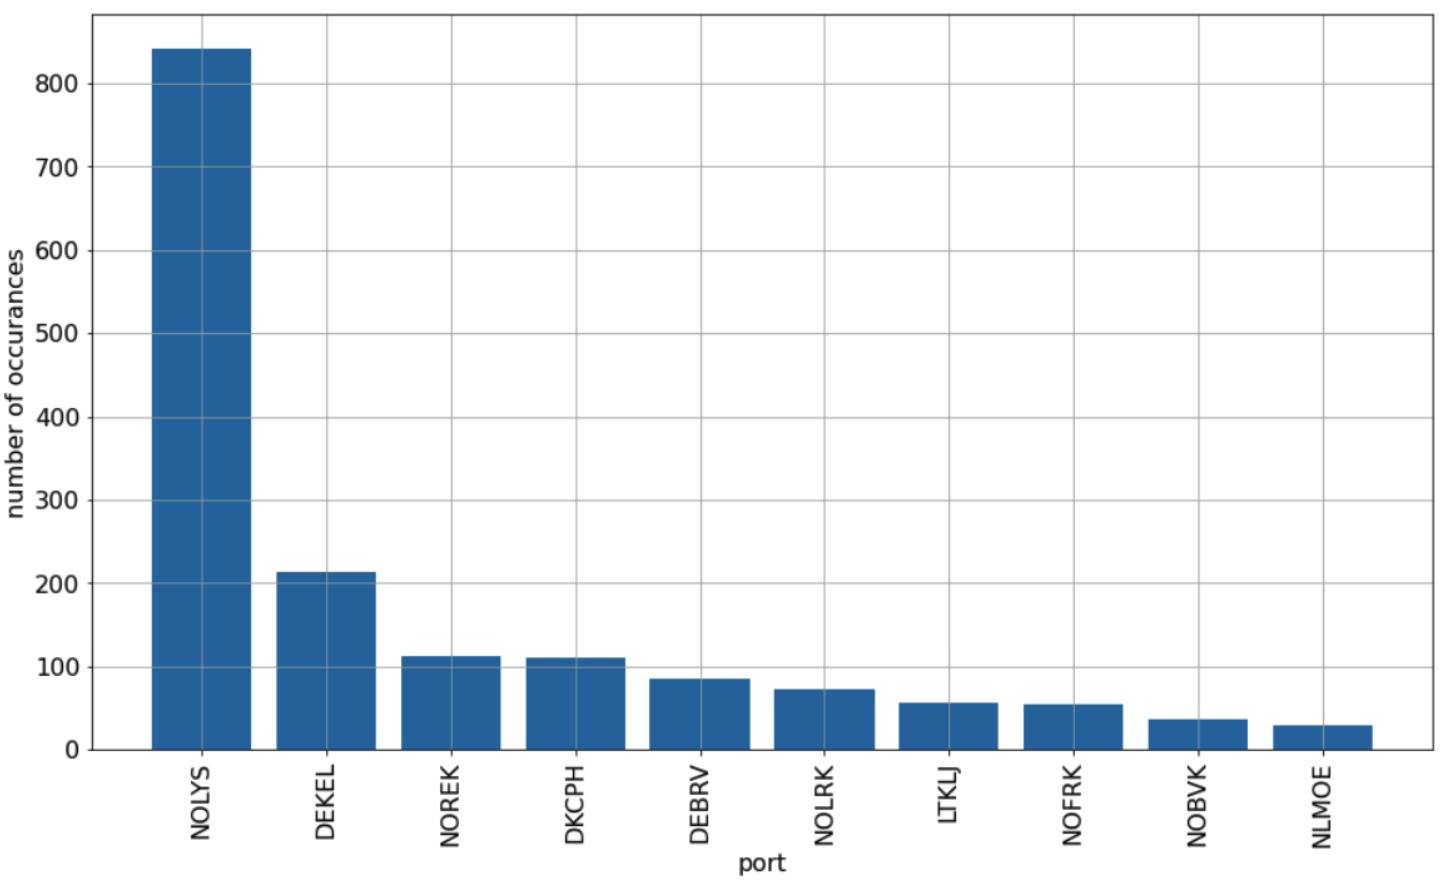
\includegraphics[width=.9\textwidth]{figures/apw/noosl_freq.png}
    \caption{Distribution of \textit{NextPort}s from \texttt{NOOSL}}
    \label{fig:apw_noosl_freq}
\end{figure}

When looking into the distributions of \textit{NextPort}s per segment it is even more apparent that the \textit{Other} segment (which includes passenger vessels) are responsible for the high number of voyages to \texttt{NOLYS}. \cref{fig:apw_noosl_segments} shows this as well as the \textit{Other} is the only segment that shares the same most frequent next port \texttt{NOLYS}. This means that a prediction algorithm using port frequencies would accurately predict the next destination ports for these other vessels, but not for the rest. Since the other vessels are responsible for 1568 out of 2009 transitions (78.05\%), considering vessel segmentation for predictions, and assuming every vessel always travel to its segment most frequent next port, a prediction algorithm could also become accurate for the remainder of the vessel segments which adds up to 21.95\% of all transition and probably most of the unique vessels. This is the basis used to estimate an improvement, or impact, factor for vessel segmentation on destination predictions.

\begin{figure}[htbp]
    \centering
    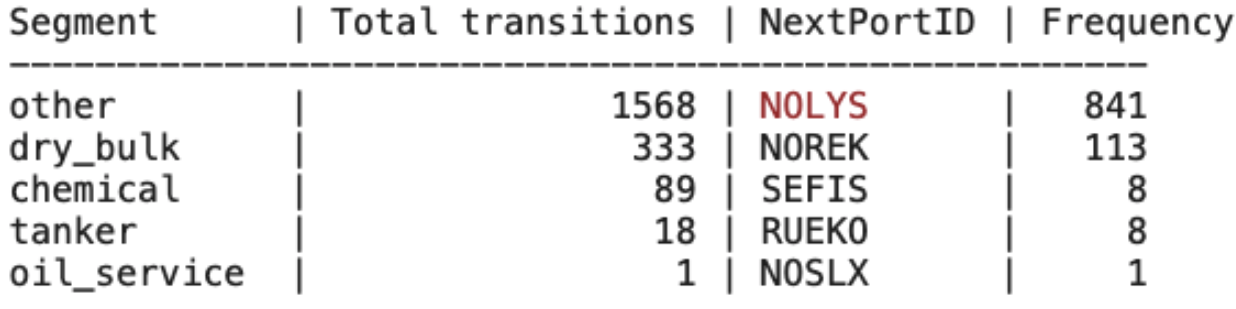
\includegraphics[width=.7\textwidth]{figures/apw/noosl_segments.png}
    \caption{Distribution of \textit{NextPort}s from \texttt{NOOSL} per segment}
    \label{fig:apw_noosl_segments}
\end{figure}

Furthermore, as \cref{fig:apw_noosl_dry_bulk} shows, when looking at the port frequency of the dry bulk cargo vessels, it is apparent that \texttt{NOLYS} is not even a contender for the most frequent next port. Therefore, a prediction method considering port frequencies would not be able to accurately predict the next destination port for any other vessel other than passenger vessels.

\begin{figure}[htbp]
    \centering
    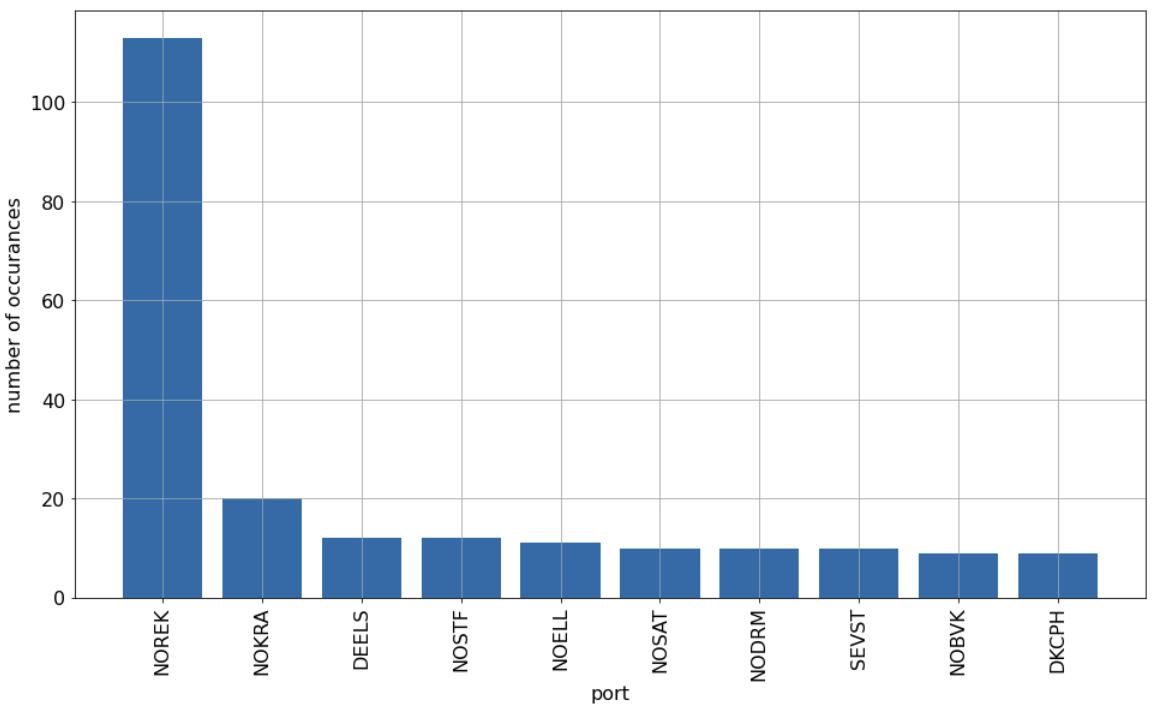
\includegraphics[width=.9\textwidth]{figures/apw/noosl_dry_bulk.png}
    \caption{Distribution of \textit{NextPort}s from \texttt{NOOSL} for the \textit{`dry bulk' segment}\label{fig:apw_noosl_dry_bulk}}
\end{figure}

Investigating sub-segments further confirms that a few numbers of vessels are responsible for most of all total transitions. \cref{fig:apw_noosl_subsegments} shows that the specific sub-segment \textit{`other - passenger'}, or passenger vessels, are responsible for 49.52\% of all transitions and nearly all voyages arrive at \texttt{NOLYS} after \texttt{NOOSL}. This means a prediction model could potentially be improved by 50\% if it would be aware of the sub-segment of each vessel for this particular port. \texttt{NOOSL} seems to be a port that shows the problem area quite well because it is a smaller port that receives a lower number of different vessels, and when there are multiple passenger vessels frequently arriving at it, they heavily skew the results in their favor.% chktex 8

\begin{figure}[htbp]
    \centering
    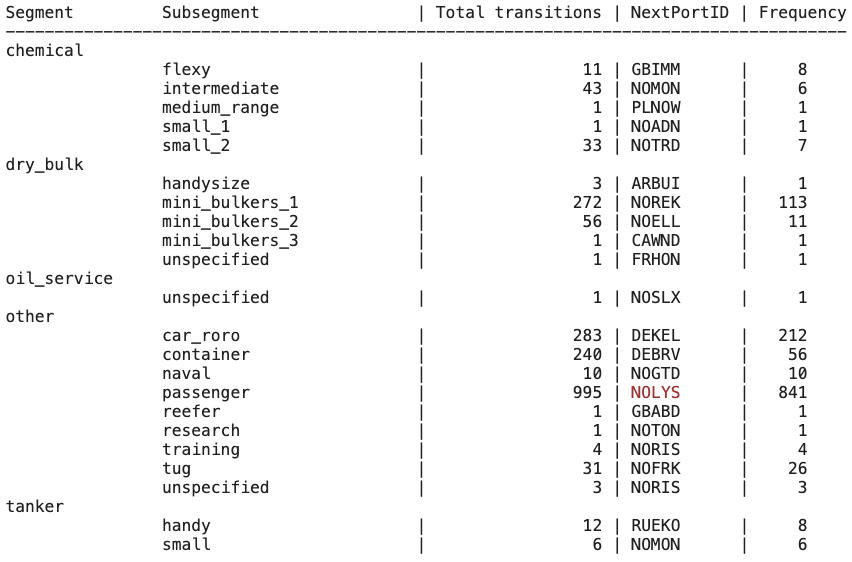
\includegraphics[width=.8\textwidth]{figures/apw/noosl_subsegments.png}
    \caption{Distribution of \textit{NextPort}s from \texttt{NOOSL} per sub-segment}
    \label{fig:apw_noosl_subsegments}
\end{figure}


\section{Trend analysis}
\label{sec:trend_analysis}

As already mentioned, for the trend analysis, a number of ports were selected based on their size and traffic. There were also a couple of known ports included in this dataset to easier interpret the results. The ports used in the analysis were:

\begin{itemize}
    \item \texttt{NLRTM} --- Rotterdam, Netherlands
    \item \texttt{NOOSL} --- Oslo, Norway
    \item \texttt{CNSHG} --- Shanghai, China
    \item \texttt{NLMSV} --- Maasvlakte, Netherlands
    \item \texttt{SGSIN} --- Singapore, Singapore
    \item \texttt{USHPY} --- Baytown, USA
    \item \texttt{BEANR} --- Antwerpen, Belgium
    \item \texttt{TWKHH} --- Kaohsiung, Taiwan
    \item \texttt{JPYOK} --- Yokohama
\end{itemize}

The same process as for the single-case analysis was conducted, but on a higher level as the main purpose of this study was to establish a trend in terms of a impact factor of vessel segmentation on port frequencies. \cref{fig:trend_freq} shows a similar version of the table used for the single port analysis (\cref{fig:apw_noosl_freq}) but also shows the number of transitions that differed from the most frequent next port when considering segments (i.e.\ the estimated improvement factor).

\begin{figure}[htbp]
    \centering
    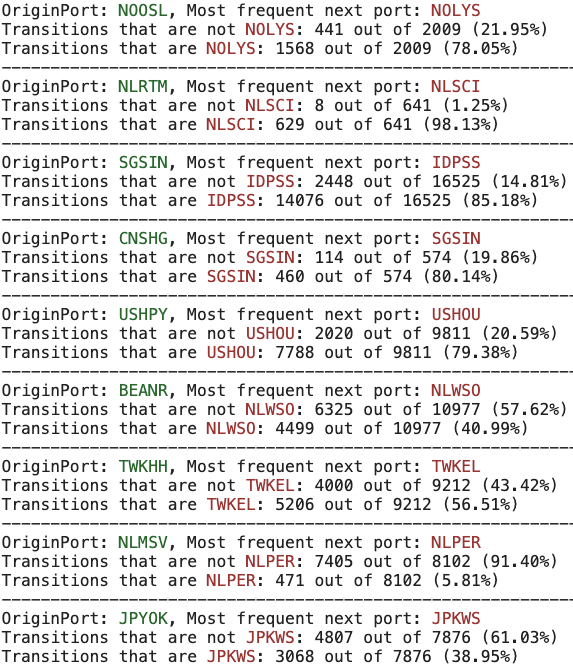
\includegraphics[width=.56\textwidth]{figures/apw/trend_frequency.png}
    \caption{Port frequencies and transition distribution as they relate to the most frequent next port for the selected ports}
    \label{fig:trend_freq}
\end{figure}

\begin{figure}[htbp]
    \centering
    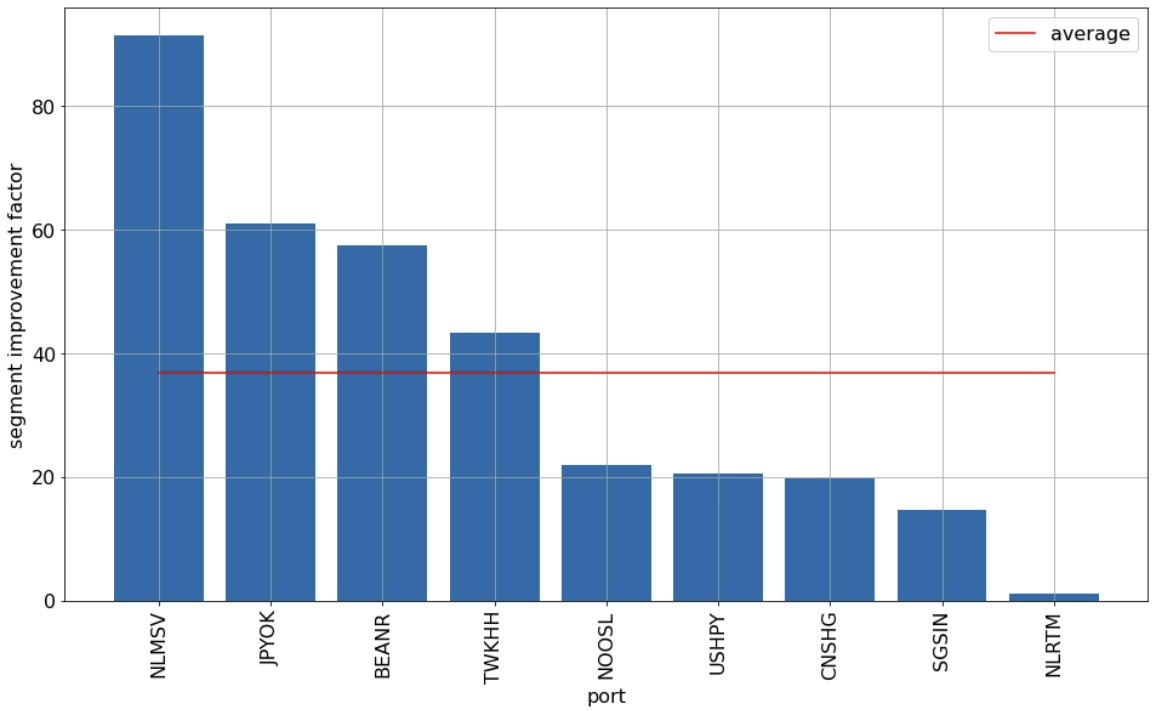
\includegraphics[width=.9\textwidth]{figures/apw/segment_improvement.png}
    \caption{Distribution of improvement factors for each origin port considering segments}
    \label{fig:segment_improvment}
\end{figure}

It is apparent that there are variances in improvement factors for different ports ranging from as low as \textit{1.25\%} to as high as \textit{91.40\%}. In the case of \texttt{NLRTM}, which is mostly a dry bulk port, there were no considerable improvements as almost all vessels are of the same segment. For the port \texttt{NLMSV}, the opposite was the case as there were a plethora of different types of vessels that frequented the port. \cref{fig:segment_improvment} shows the distribution of the improvement factor considering segments for each origin port as well as the overall average impact factor for these 9 ports which was \textit{36.88\%}.

Furthermore, when looking at the impact of sub-segments, as \cref{fig:subsegment_improvment} shows, it seems that the improvement factor has increased overall. For example, in the case of \texttt{NLRTM}, the improvement factor has increased from \textit{1.25\%} to \textit{19.66\%}, and although this varied for the different ports, the overall average improvement factor increased from \textit{36.88\%} to \textit{50.28\%}.

\begin{figure}[htbp]
    \centering
    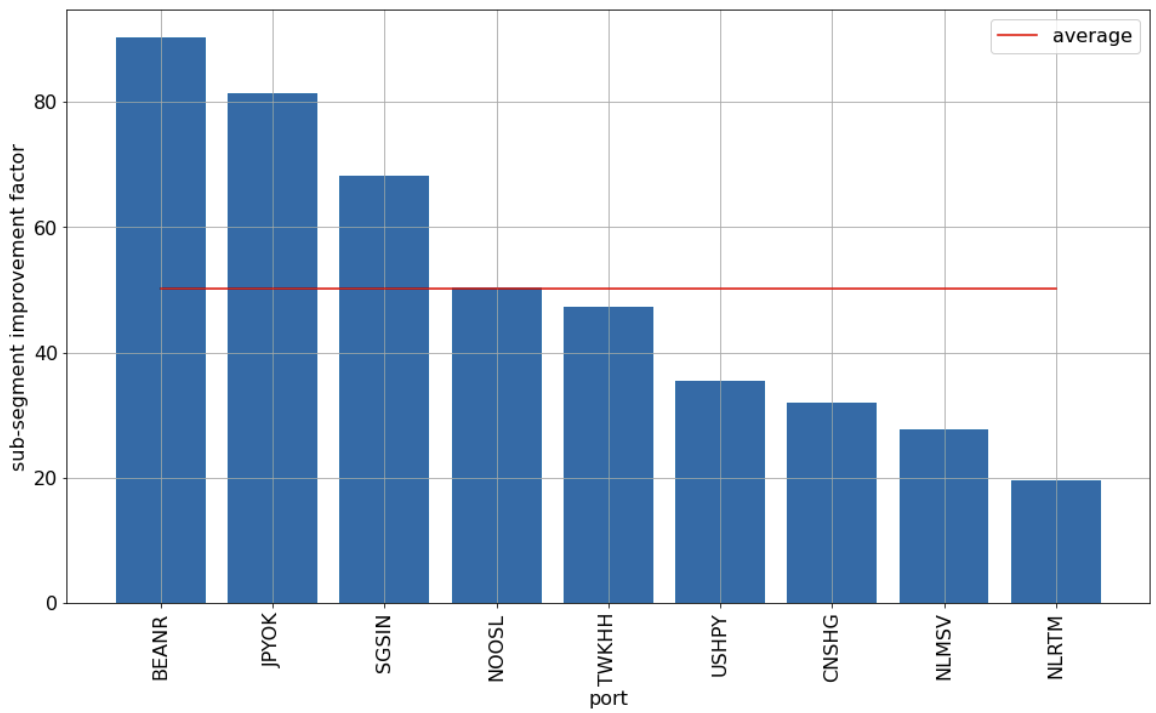
\includegraphics[width=.9\textwidth]{figures/apw/subsegment_improvement.png}
    \caption{Distribution of improvement factors for each origin port considering sub-segments}
    \label{fig:subsegment_improvment}
\end{figure}

A prediction method considering the frequencies of ports for vessel destination predictions would choose the most frequent next port for the predicted next destination. In this scenario, ignoring the vessel's type (segmentation) would give the wrong prediction for a lot of vessels from different segments in a lot of ports. The results from the feasibility study clearly indicates that applying the aspect of vessel segmentation to such models would definitively have an impact on prediction accuracy and, therefore, is worth investigating further. Moreover, assuming this impact would also, to some degree, apply to vessel trajectories as they relate to traveling patters, improving the accuracy of a model such as the one described in~\cite{Zhang2020AISApproach} seems to be plausible depending on the data foundation.

\chapter{Methodology}

\section{Processed dataset used for analysis}

\subsection{Vessel position history}

\begin{itemize}
    \item Validated on geographical coordinates
    \item Validated on MMSI -> IMO mapping and valid values
    \item Filtered from 1 billion to 450 million etc...
    \item Visualization ?
\end{itemize}

\subsection{Vessel transitions}

 - A direct copy of MO's
 
 \subsection{Ports}
 
 - A direct copy of MO's "visible" ports
 
 \subsection{Segments}
 
 - A direct copy of MO's
 
 \subsection{Transition voyages}
 
 \subsection{Clustered voyages}
 
\chapter{Results}

\chapter{Discussion}


\chapter*{\bibname}
\printbibliography[heading=none]

% First paper

\begin{paper}{papers/landes1951scrutiny.pdf}{paper:scrutiny}
    Here, you may add a description of the paper, an illustration, or just give the bibliographic reference:
    \begin{quote}
        hello world
    \end{quote}
    Or you may leave it empty, if you like.
\end{paper}

% Second paper etc.

\appendix
\chapter{Additional Material}
\label{app:additional}

Additional material that does not fit in the main thesis but may still be relevant to share, e.g., raw data from experiments and surveys, code listings, additional plots, pre-project reports, project agreements, contracts, logs etc., can be put in appendices. Simply issue the command \texttt{\textbackslash appendix} in the main \texttt{.tex} file, and make one chapter per appendix.

If the appendix is in the form of a ready-made PDF file, it should be supported by a small descriptive text, and included using the \texttt{pdfpages} package. To illustrate how it works, a standard project agreement (for the IE faculty at NTNU in Gjøvik) is attached here. You would probably want the included PDF file to begin on an odd (right hand) page, which is achieved by using the \texttt{\textbackslash cleardoublepage} command immediately before the \texttt{\textbackslash includepdf[]\{\}} command. Use the option \texttt{[pages=-]} to include all pages of the PDF document, or, e.g., \texttt{[pages=2-4]} to include only the given page range.


\end{document}
